\documentclass[10pt]{beamer}
\usepackage[UTF8]{ctex}
\usepackage{natbib}
\usepackage{commath}%定义d
\usepackage{graphicx}
\graphicspath{{fig/}}
\usepackage{booktabs} % To thicken table lines
\usepackage{bm}
\usepackage{cleveref}
\usepackage{hyperref}

\usepackage{amsmath,amssymb,enumerate,color}
\usepackage{graphicx,listings}

\newcommand\mi{\mathrm{i}}
\newcommand\me{\mathrm{e}}
\usetheme[progressbar=frametitle]{metropolis}

\setsansfont{TimesNewRomanPSMT}
\setmonofont{SFMono-Regular}
\setmainfont{TimesNewRomanPSMT}

\title{Matlab 第六章\quad 代数方程与最优化问题的计算机求解}
\author{\footnotesize 袁磊祺 \quad 刘志如 \quad 宋庭鉴  \quad 周子铭 \quad 岐亦铭 \quad 董淏翔 \quad  撒普尔}
\date{\today}
%\logo{
\includegraphics[width=5em]{pkured.pdf}}

\setCJKmainfont[ItalicFont=STKaitiSC-Regular,BoldFont=STSongti-SC-Black]{STSongti-SC-Regular}
\setCJKsansfont[ItalicFont=STKaitiSC-Regular,BoldFont=STHeitiSC-Medium]{STHeitiSC-Light}

\definecolor{light-gray}{gray}{0.95} 
\lstset{ %
	backgroundcolor=\color{light-gray},   % choose the background color
	basicstyle=\scriptsize\rmfamily,     % size of fonts used for the code
	columns=fullflexible,
	breaklines=true,                 % automatic line breaking only at whitespace
	captionpos=b,                    % sets the caption-position to bottom
}

\begin{document}
  %%%%%%%%%%%%%%%%%%%%%%%%%%%%%%%%%%%%%%%%%%%%%%
\renewcommand\contentsname{\vspace*{-2cm}\centerline{\textsf{目\quad 录}}\vspace*{-1.5cm}}
\renewcommand\listfigurename{插图目录}
\renewcommand\listtablename{表格目录}
\renewcommand\refname{参考文献}
\renewcommand\indexname{索引}
\renewcommand\figurename{图}
\renewcommand\tablename{表}
\renewcommand\abstractname{摘\quad 要}
\renewcommand\partname{部分}
\renewcommand\appendixname{附录}
\def\equationautorefname{式}%
\def\footnoteautorefname{脚注}%
\def\itemautorefname{项}%
\def\figureautorefname{图}%
\def\tableautorefname{表}%
\def\partautorefname{篇}%
\def\appendixautorefname{附录}%
\def\chapterautorefname{章}%
\def\sectionautorefname{节}%
\def\subsectionautorefname{小小节}%
\def\subsubsectionautorefname{subsubsection}%
\def\paragraphautorefname{段落}%
\def\subparagraphautorefname{子段落}%
\def\FancyVerbLineautorefname{行}%
\def\theoremautorefname{定理}%
\crefname{figure}{图}{图}
\crefname{equation}{式}{式}
\crefname{table}{表}{表}



  \maketitle
  \begin{frame}
		\frametitle{目录}
		\tableofcontents{}
\end{frame}

% qym


\section{代数方程的求解}
	% \subsection{代数方程的图解法}
\begin{frame}[fragile]{一元方程的图解法}
		  	\textbf{思路:}用ezplot()函数绘隐函数$f(x)=0$曲线找零点。
			 \begin{example}[6-1]
				解$\mathrm{e}^{-3 t} \sin (4 t+2)+4 \mathrm{e}^{-0.5 t} \cos (2 t)=0.5$。

		  	\begin{columns}[T]
			  		\column{.4\textwidth}
			  	\begin{block}{MATLAB代码:}
    \begin{lstlisting}
figure
ezplot('exp(-3*t)*sin(4*t+2)+4*exp(-0.5*t)*cos(2*t)-.5',[0 5])
line([0,5],[0,0])
    \end{lstlisting}	
			\end{block}	  		
		  		\column{.6\textwidth}
				\begin{block}{输出:}
					\centering
					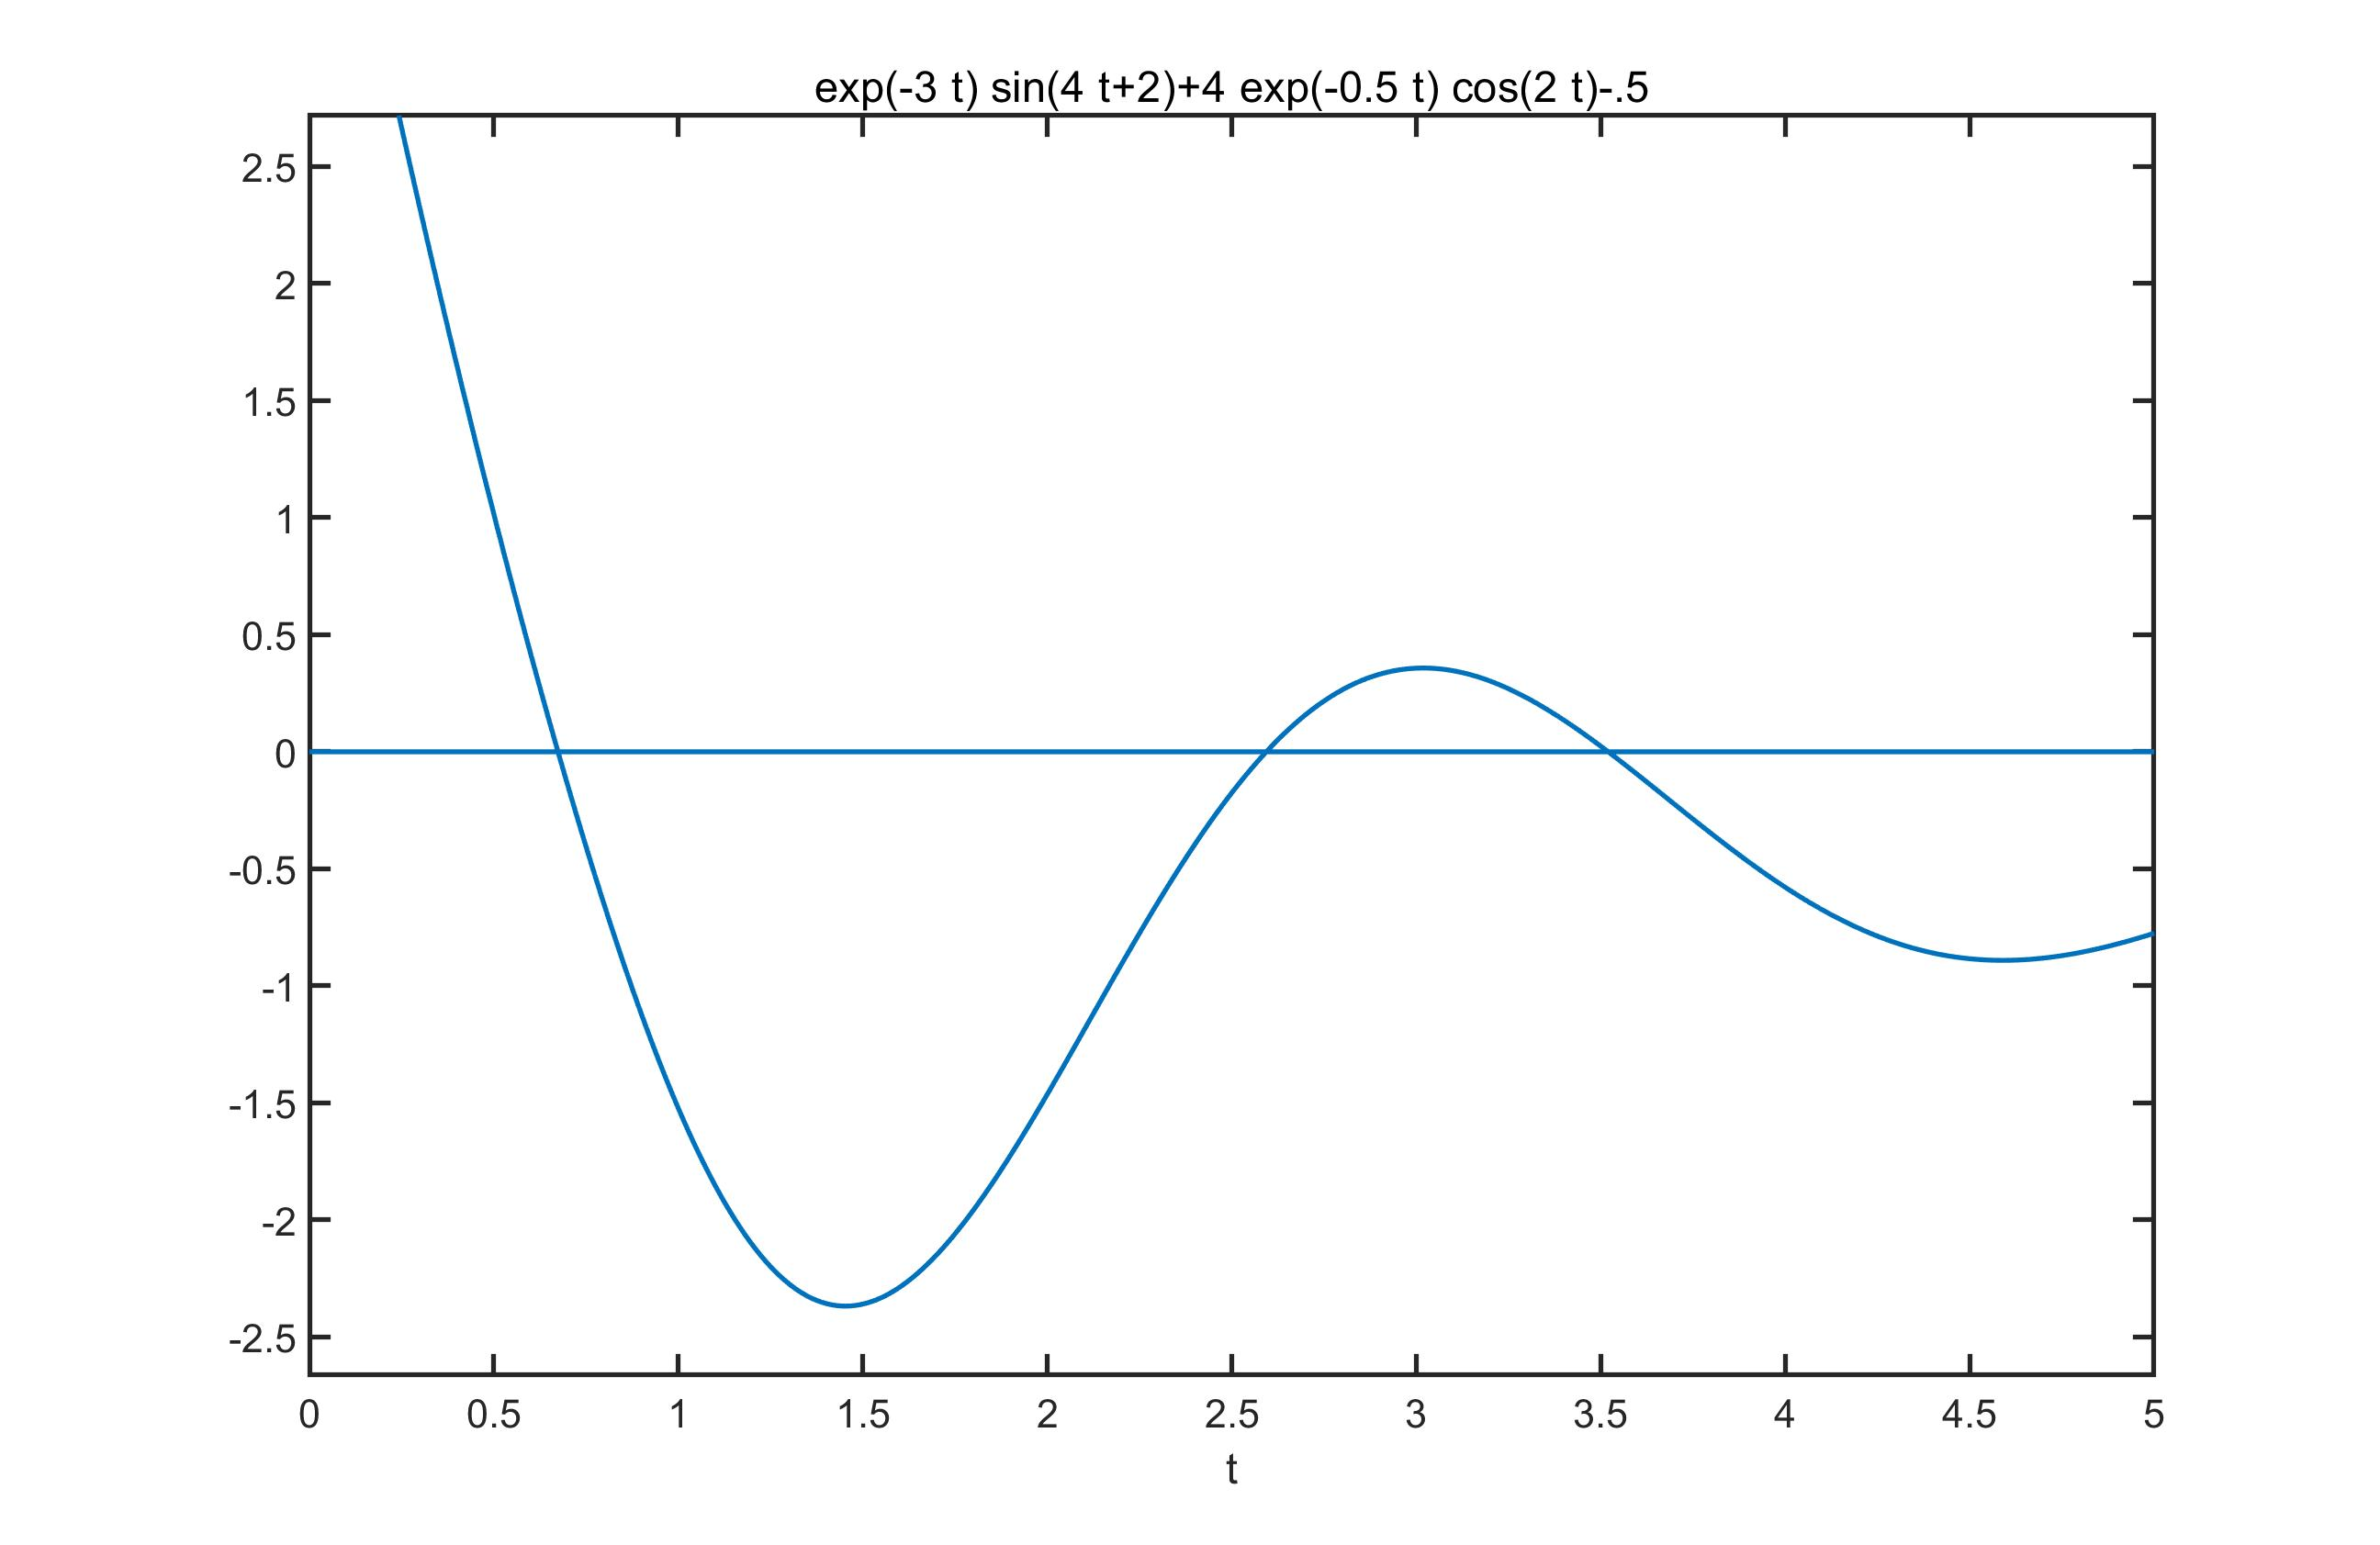
\includegraphics[width=\textwidth]{11}
				 \end{block}
		  	\end{columns}
三个解,约为0.670、2.59、3.51.
		\end{example}
\end{frame}
%---------------------------------------------------------------------- 	
\begin{frame}[fragile]{二元方程的图解法}
		\textbf{思路:}绘制在同一张图上看交点。
	\begin{example}[6-2]解
		$\left\{\begin{array}{l}
		x^{2} \mathrm{e}^{-x y^{2} / 2}+\mathrm{e}^{-x / 2} \sin (x y)=0 \\
		x^{2} \cos \left(x+y^{2}\right)+y^{2} \mathrm{e}^{x+y}=0
		\end{array}\right.$
	
		\begin{columns}[T]
			\column{.4\textwidth}
				\begin{block}{MATLAB代码:}
\begin{lstlisting}
figure
ezplot('x^2*exp(-x*y^2/2)+exp(-x/2)*sin(x*y)')
hold on
h1 = ezplot('y^2*cos(y+x^2)+x^2*exp(x+y)');
set(h1,'Color','k')
hold off
\end{lstlisting}
				\end{block}	  		
		
			\column{.6\textwidth}
				\begin{block}{输出:}
					\centering
					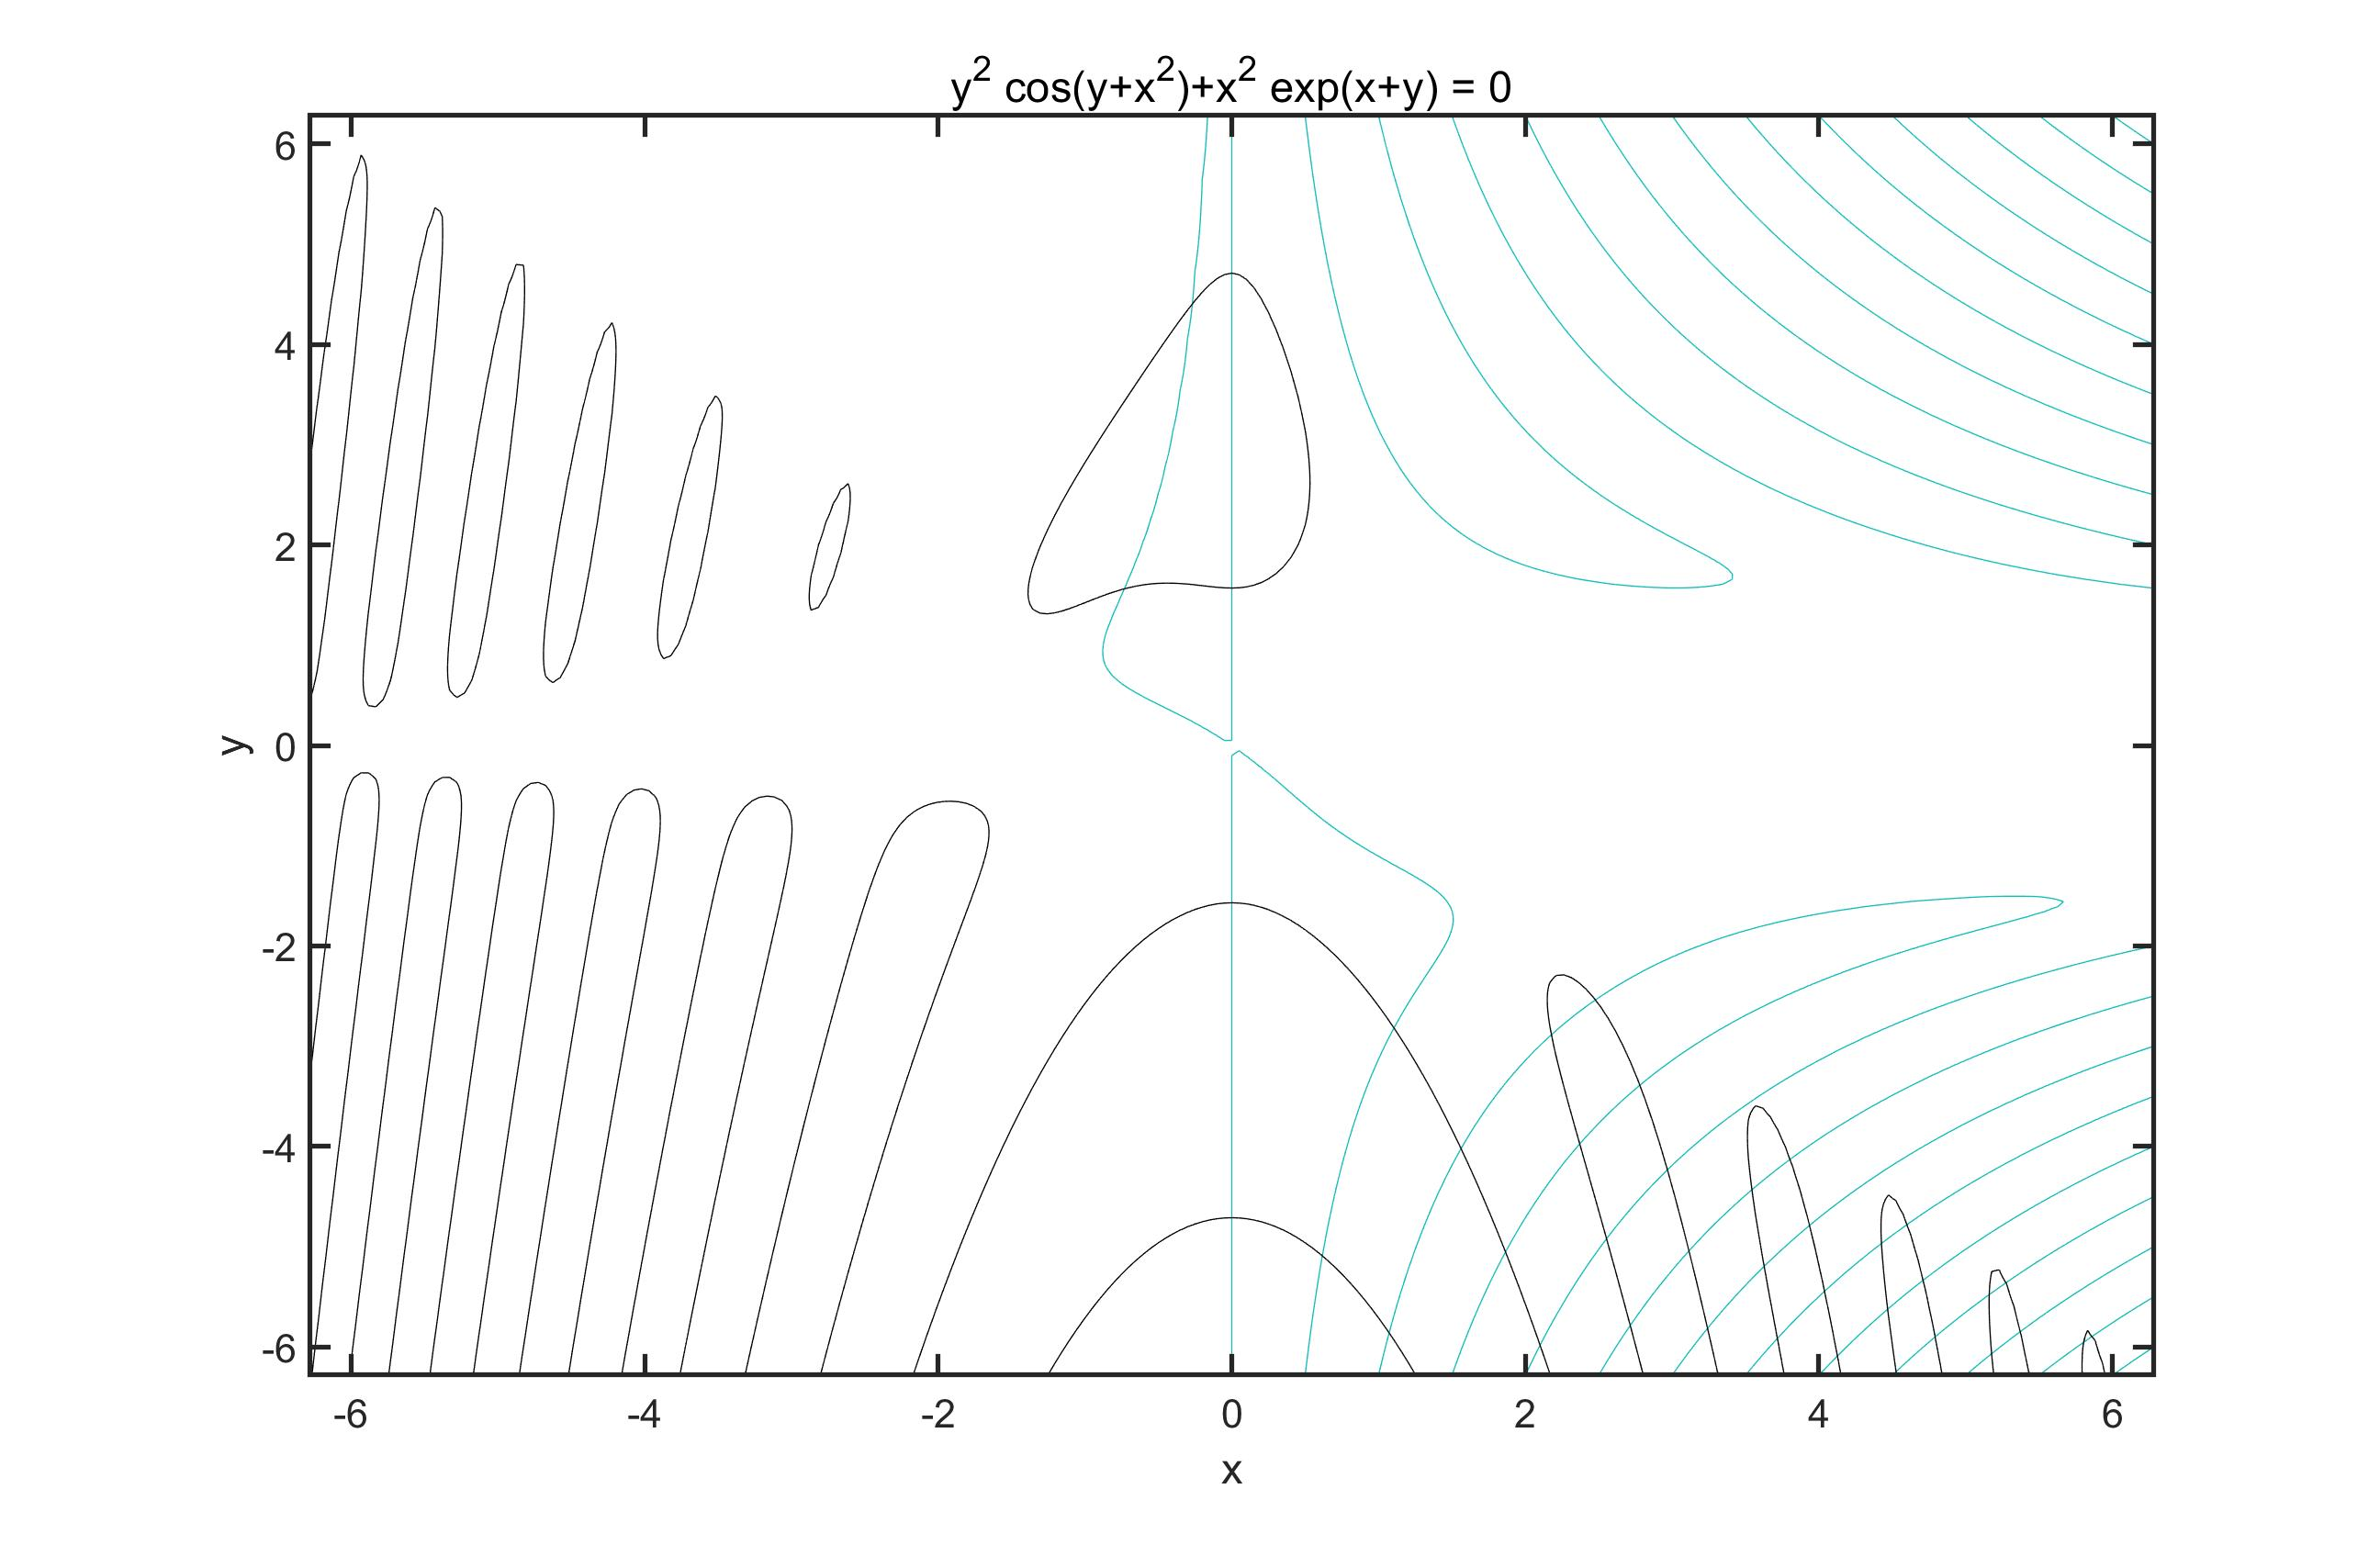
\includegraphics[width=\textwidth]{12}
				\end{block}
		\end{columns}
	\end{example}

	\textbf{局限:}
仅适用\textbf{一元、二元}方程。
仅能\textbf{近似}得\textbf{实数}根。

\end{frame}
%---------------------------------------------------------------------- 
	% \subsection{多项式型方程的准解析解法}
		\begin{frame}[fragile]{多项式型方程的准解析解法}
		\begin{block}{用solve函数,语法:}
\begin{lstlisting}
S = solve(eqn1, eqn2,... ,eqnn)%最简调用方式
[x,...] = solve(eqn1, eqn2,... ,eqnn)%直接得出根
[x,...] = solve(eqn1, eqn2,... ,eqnn, 'x,...')%同上, 并指定变量
\end{lstlisting}
		\end{block}	  
		\begin{columns}[T]
			\column{.7\textwidth}
		\begin{example}[6-4]
			解$\left\{\begin{array}{l}
			x^{2}+y^{2}-1=0 \\
			0.75 x^{3}-y+0.9=0
			\end{array}\right.$
		\end{example}
	\begin{block}{MATLAB代码:}
\begin{lstlisting}
syms x y
[x,y]=solve(x^2+y^2-1==0,0.75*x^3-y+0.9==0)
x=double(x), y=double(y)
[eval('x.^2+y.^2-1') eval('0.75*x.^3-y+0.9')]%解的验算
\end{lstlisting}
	\end{block}
			\column{.3\textwidth}
		\begin{block}{输出:}
\begin{lstlisting}
x = -0.9817 + 0.0000i
    0.3570 + 0.0000i
    -0.5540 - 0.3547i
    -0.5540 + 0.3547i
    0.8663 - 1.2154i
    0.8663 + 1.2154i
y = 0.1904 + 0.0000i
    0.9341 + 0.0000i
    0.9293 - 0.2114i
    0.9293 + 0.2114i
    -1.4916 - 0.7059i
    -1.4916 + 0.7059i
\end{lstlisting}	
		\end{block}			
	\end{columns}
		\end{frame}
%---------------------------------------------------------------------- 
	% \subsection{一般非线性方程数值解}
		\begin{frame}[fragile]{一般非线性方程数值解}
	\begin{block}{用fsolve()函数,语法:}
\begin{lstlisting}
x = fsolve(fun,x0)%最简单求解语句
[x,f,flag,out] = fsolve(fun,x0,opt,p1,p2,...)%一般求解格式
opt = optimset%获得默认的常用变量
opt.TolX=1e-10; set(opt,'TolX',1e-10)%修改参数
\end{lstlisting}
	\end{block}	  

	\begin{example}[6-8]
解Lambert函数,其解$w$满足$we^{w} = x$。
	\end{example}

	\begin{block}{MATLAB代码:}
		\begin{columns}[T]
	\column{.5\textwidth}
\begin{lstlisting}
figure
y=[]; xx=0:.05:10; x0=0; h=optimset; h.Display='off';
for x = xx
y1 = fsolve(@(w) w.*exp(w)-x,x0,h); x0=y1; y=[y,y1];
end
\end{lstlisting}

	\column{.5\textwidth}
\begin{lstlisting}
subplot(2,1,1);
plot(xx,y);
y0 = lambertw(xx);
subplot(2,1,2);
plot(xx,y0,'r');
\end{lstlisting}
		\end{columns}
	\end{block}
\end{frame}
%---------------------------------------------------------------------- 
\begin{frame}[fragile]{一般非线性方程数值解}
	\begin{block}{输出:}
		\centering
		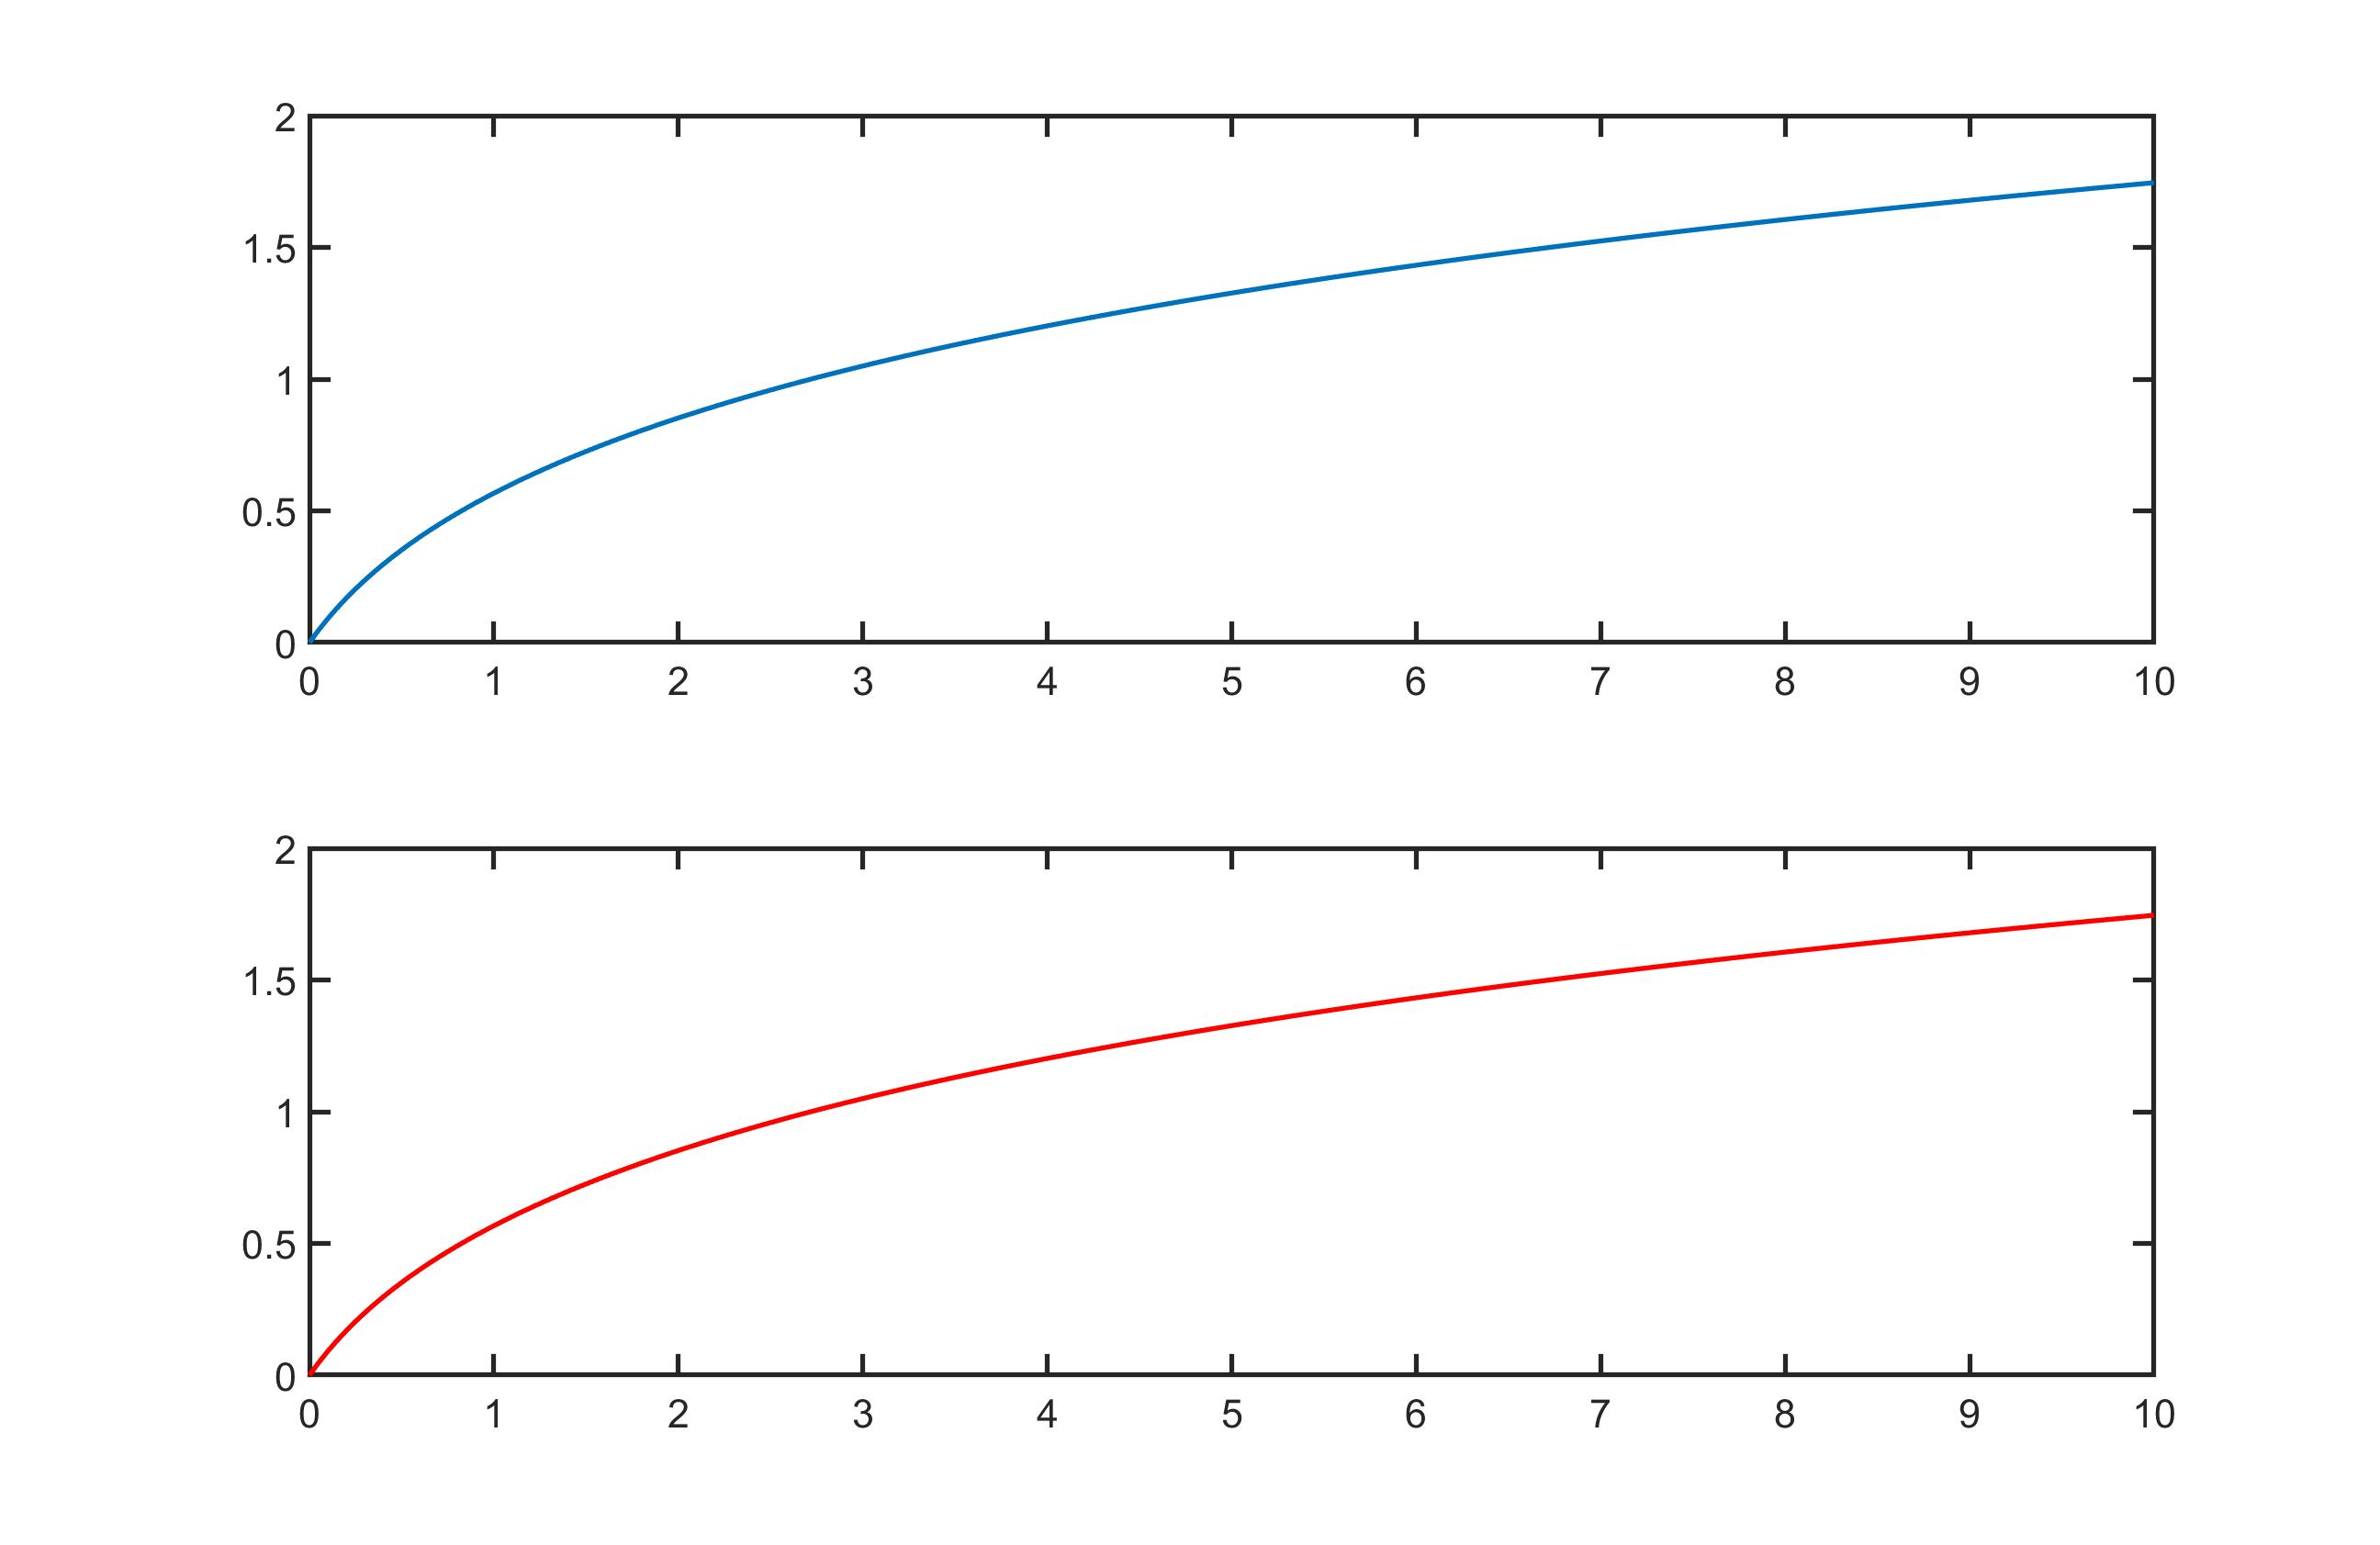
\includegraphics[width=.7\textwidth]{13}
		
		{\color{cyan}蓝线}:fsolve()的解,{\color{red}红线}:软件自带该问题求值函数。
	\end{block}		
\end{frame}
%---------------------------------------------------------------------- 
\section{无约束最优化问题求解}
	% \subsection{解析解法与图解法}
		\begin{frame}[fragile]{解析解法与图解法}
\textbf{无约束最优化问题提法:}$\min\limits_{x} f(\mathbf{x})$,优化变量$\mathbf{x} = [x_1,...,x_n]^T$,目标函数$f(\cdot)$。

\textbf{解析解法:}最优点出现在一阶导数为零的点上,可列$
\left.\frac{\partial f}{\partial x_{1}}\right|_{\mathbf{x}=\mathbf{x}^{*}}=0,\left.\frac{\partial f}{\partial x_{2}}\right|_{\mathbf{x}=\mathbf{x}^{*}} 0, \cdots,\left.\frac{\partial f}{\partial x_{n}}\right|_{\mathbf{x}=\mathbf{x}^{*}}=0$

$
\Longrightarrow
\left\{\begin{array}{l}
\text{高数:Hessian矩阵。} \\
\text{\textbf{图解法:}画曲线判断极值点。} {\color{red}\checkmark}
\end{array}\right.
$
			
\textbf{局限:}一元、二元函数适用,三元或多元函数无法画图表示。
		\end{frame}
%---------------------------------------------------------------------- 
\begin{frame}[fragile]{解析解法与图解法}
\begin{columns}[T]
	\column{.4\textwidth}
		\begin{example}[6-11]
			讨论例6-1函数最优性。
		\end{example}
		\begin{block}{MATLAB代码:}
\begin{lstlisting}
syms t
y = exp(-3*t)*sin(4*t+2)+4*exp(-0.5*t)*cos(2*t)-.5;
y1 = diff(y,t)
t0 = solve(y1)
b = subs(diff(y1),t,t0)
\end{lstlisting}			
		\end{block}
		
	\column{.6\textwidth}
		\begin{block}{输出:}
			\centering
			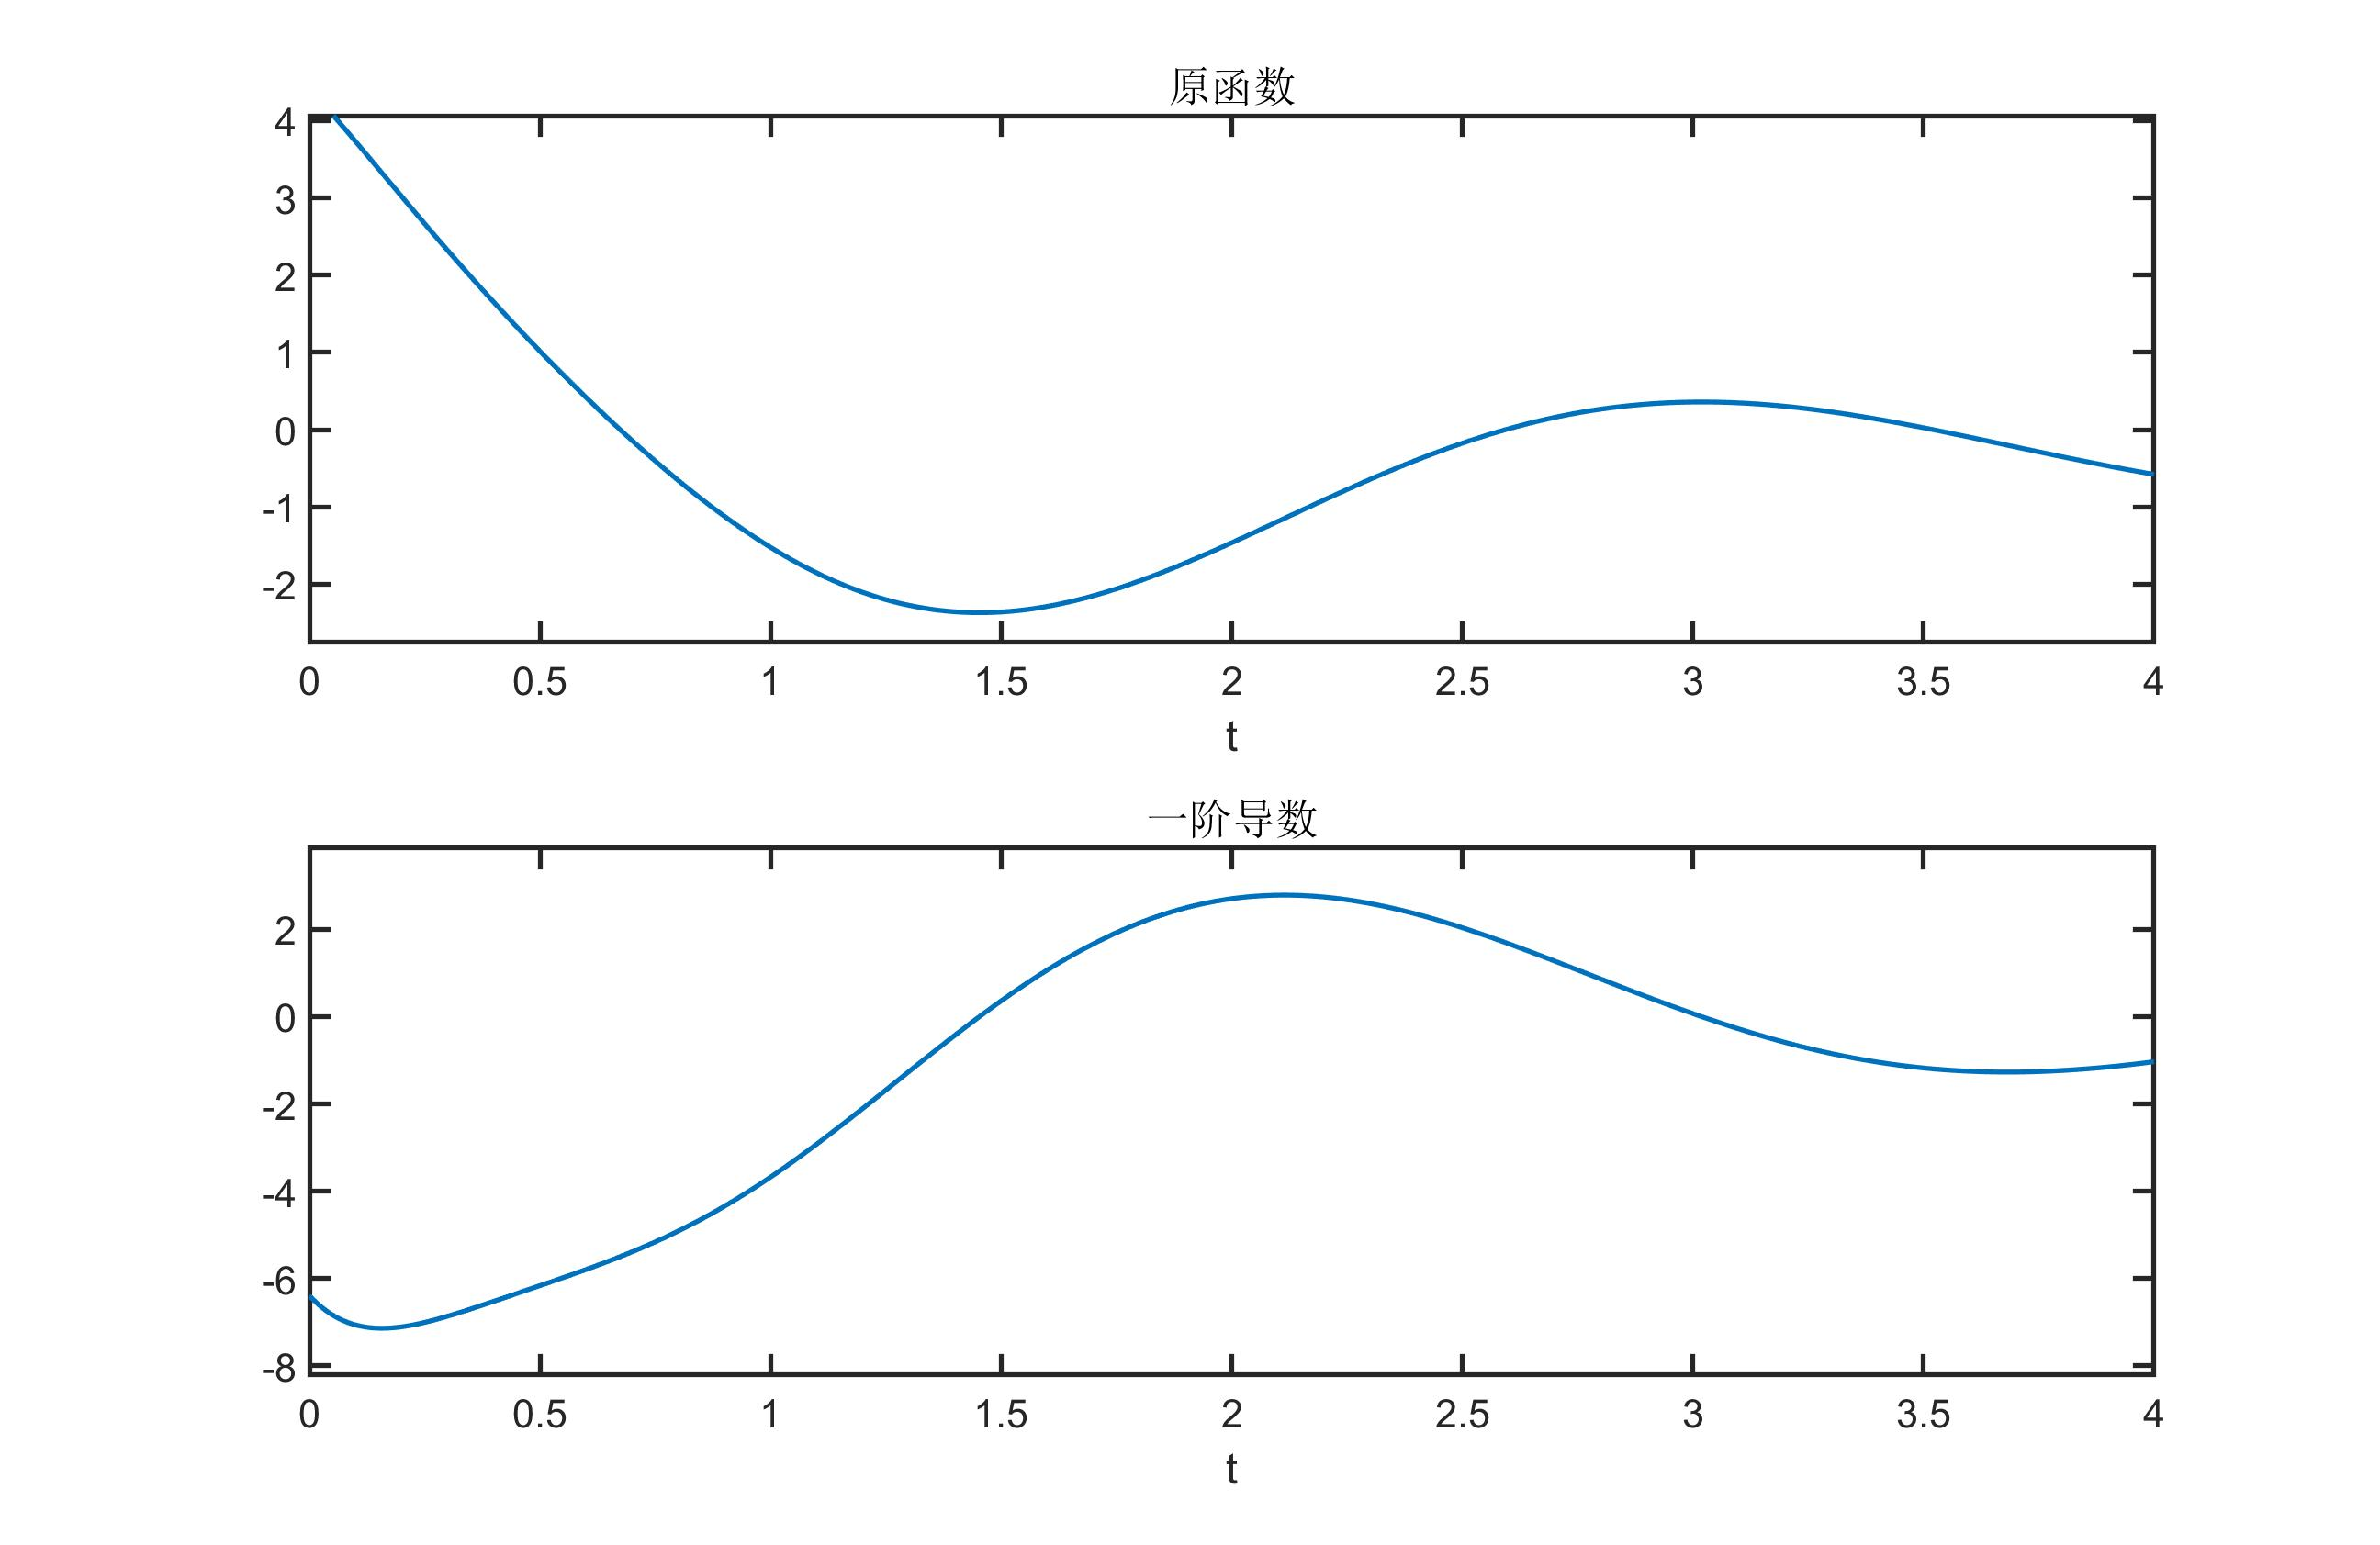
\includegraphics[width=\textwidth]{22}
			
			可见在[0,4]内约1.46处,最小值约-2.37。
		\end{block}
\end{columns}
\end{frame}
%---------------------------------------------------------------------- 
	% \subsection{基于MATLAB的数值解法}
		\begin{frame}[fragile]{基于MATLAB的数值解法}
			\textbf{数学原理:}单纯形(Simplex)法。{\scriptsize(Def: N dim., N+1 vertices interconnect)}
			
			\textbf{思路:}调用fminsearch()或者fminunc()函数。
			
			\begin{block}{调用语法,fminunc()为例:}
\begin{lstlisting}
x=fminunc(Fun, x0) %最简求解语句
[x,f,flag,out]=fminunc(Fun, x0, opt, p1, p2,...) %一般求解格式
\end{lstlisting}
			\end{block}	  
		
		\begin{example}[6-12]
求$z=f(x, y)=\left(x^{2}-2 x\right) \mathrm{e}^{-x^{2}-y^{2}-x y}$最小值。
		\end{example}
			
			\begin{block}{MATLAB代码:}
\begin{lstlisting}
ff2=@(x)(x(1)^2-2*x(1))*exp(-x(1)^2-x(2)^2-x(1)*x(2));
ff2_0 = optimset;
ff2_0.Display='iter';
result1 = fminsearch(ff2,[0; 0],ff2_0)
result2 = fminunc(ff2,[0; 0],ff2_0)
\end{lstlisting}
			\end{block}	 
		
		\end{frame}
	
%---------------------------------------------------------------------- 
\begin{frame}[t,fragile]{fminsearch输出}
		
		\begin{lstlisting}
Iteration   Func-count     min f(x)         Procedure
0           1                0         
1           3     -0.000499937         initial simplex
2           4     -0.000499937         reflect
3           6      -0.00149944         expand
4           7      -0.00149944         reflect
......
71          135        -0.641424         contract inside
72          137        -0.641424         contract outside
......
优化已终止:当前的 x 满足使用 1.000000e-04 的 OPTIONS.TolX 的终止条件,F(X) 满足使用 1.000000e-04 的 OPTIONS.TolFun 的收敛条件
......
result1 =
0.6111
-0.3056
\end{lstlisting}
		
\end{frame}

%---------------------------------------------------------------------- 
\begin{frame}[t,fragile]{fminunc输出}

\begin{lstlisting}
Iteration  Func-count       f(x)        Step-size       First-order optimality
0           3                0                             2
1           6        -0.367879            0.5          0.736  
......
6          24        -0.641424              1       0.000619  
7          27        -0.641424              1        1.8e-06
......
Optimization completed because the size of the gradient is less than the value of the optimality tolerance.
......
result2 =
0.6110
-0.3055
\end{lstlisting}

\end{frame}

%----------------------------------------------------------------------
 
	% \subsection{全局最优解与局部最优解}
\begin{frame}[fragile]{全局最优解与局部最优解}
	\textbf{概念:}导数为0的点包括局部和全局最优点。得到的最优点依赖于初始选取。$\Leftarrow$可以用遗传算法试不同初值
	
	\begin{columns}[T]
		\column{.4\textwidth}
		
	\begin{example}[6-13]
		$y(t)=\mathrm{e}^{-2 t} \cos 10 t+\mathrm{e}^{-3 t-6} \sin 2 t, t \geqslant 0$局部最小值与全局最小值。
	\end{example}
	
	\begin{block}{MATLAB代码:}
\begin{lstlisting}
ff3=@(t)exp(-2*t).*cos(10*t)+exp(-3*(t+2)).*sin(2*t);
[t3_1,f3_1] = fminsearch(ff3,1)
[t3_2,f3_2] = fminsearch(ff3,.1)
\end{lstlisting}
	\end{block}	
	
		\column{.65\textwidth}
		
		\begin{block}{输出:}
	\centering
	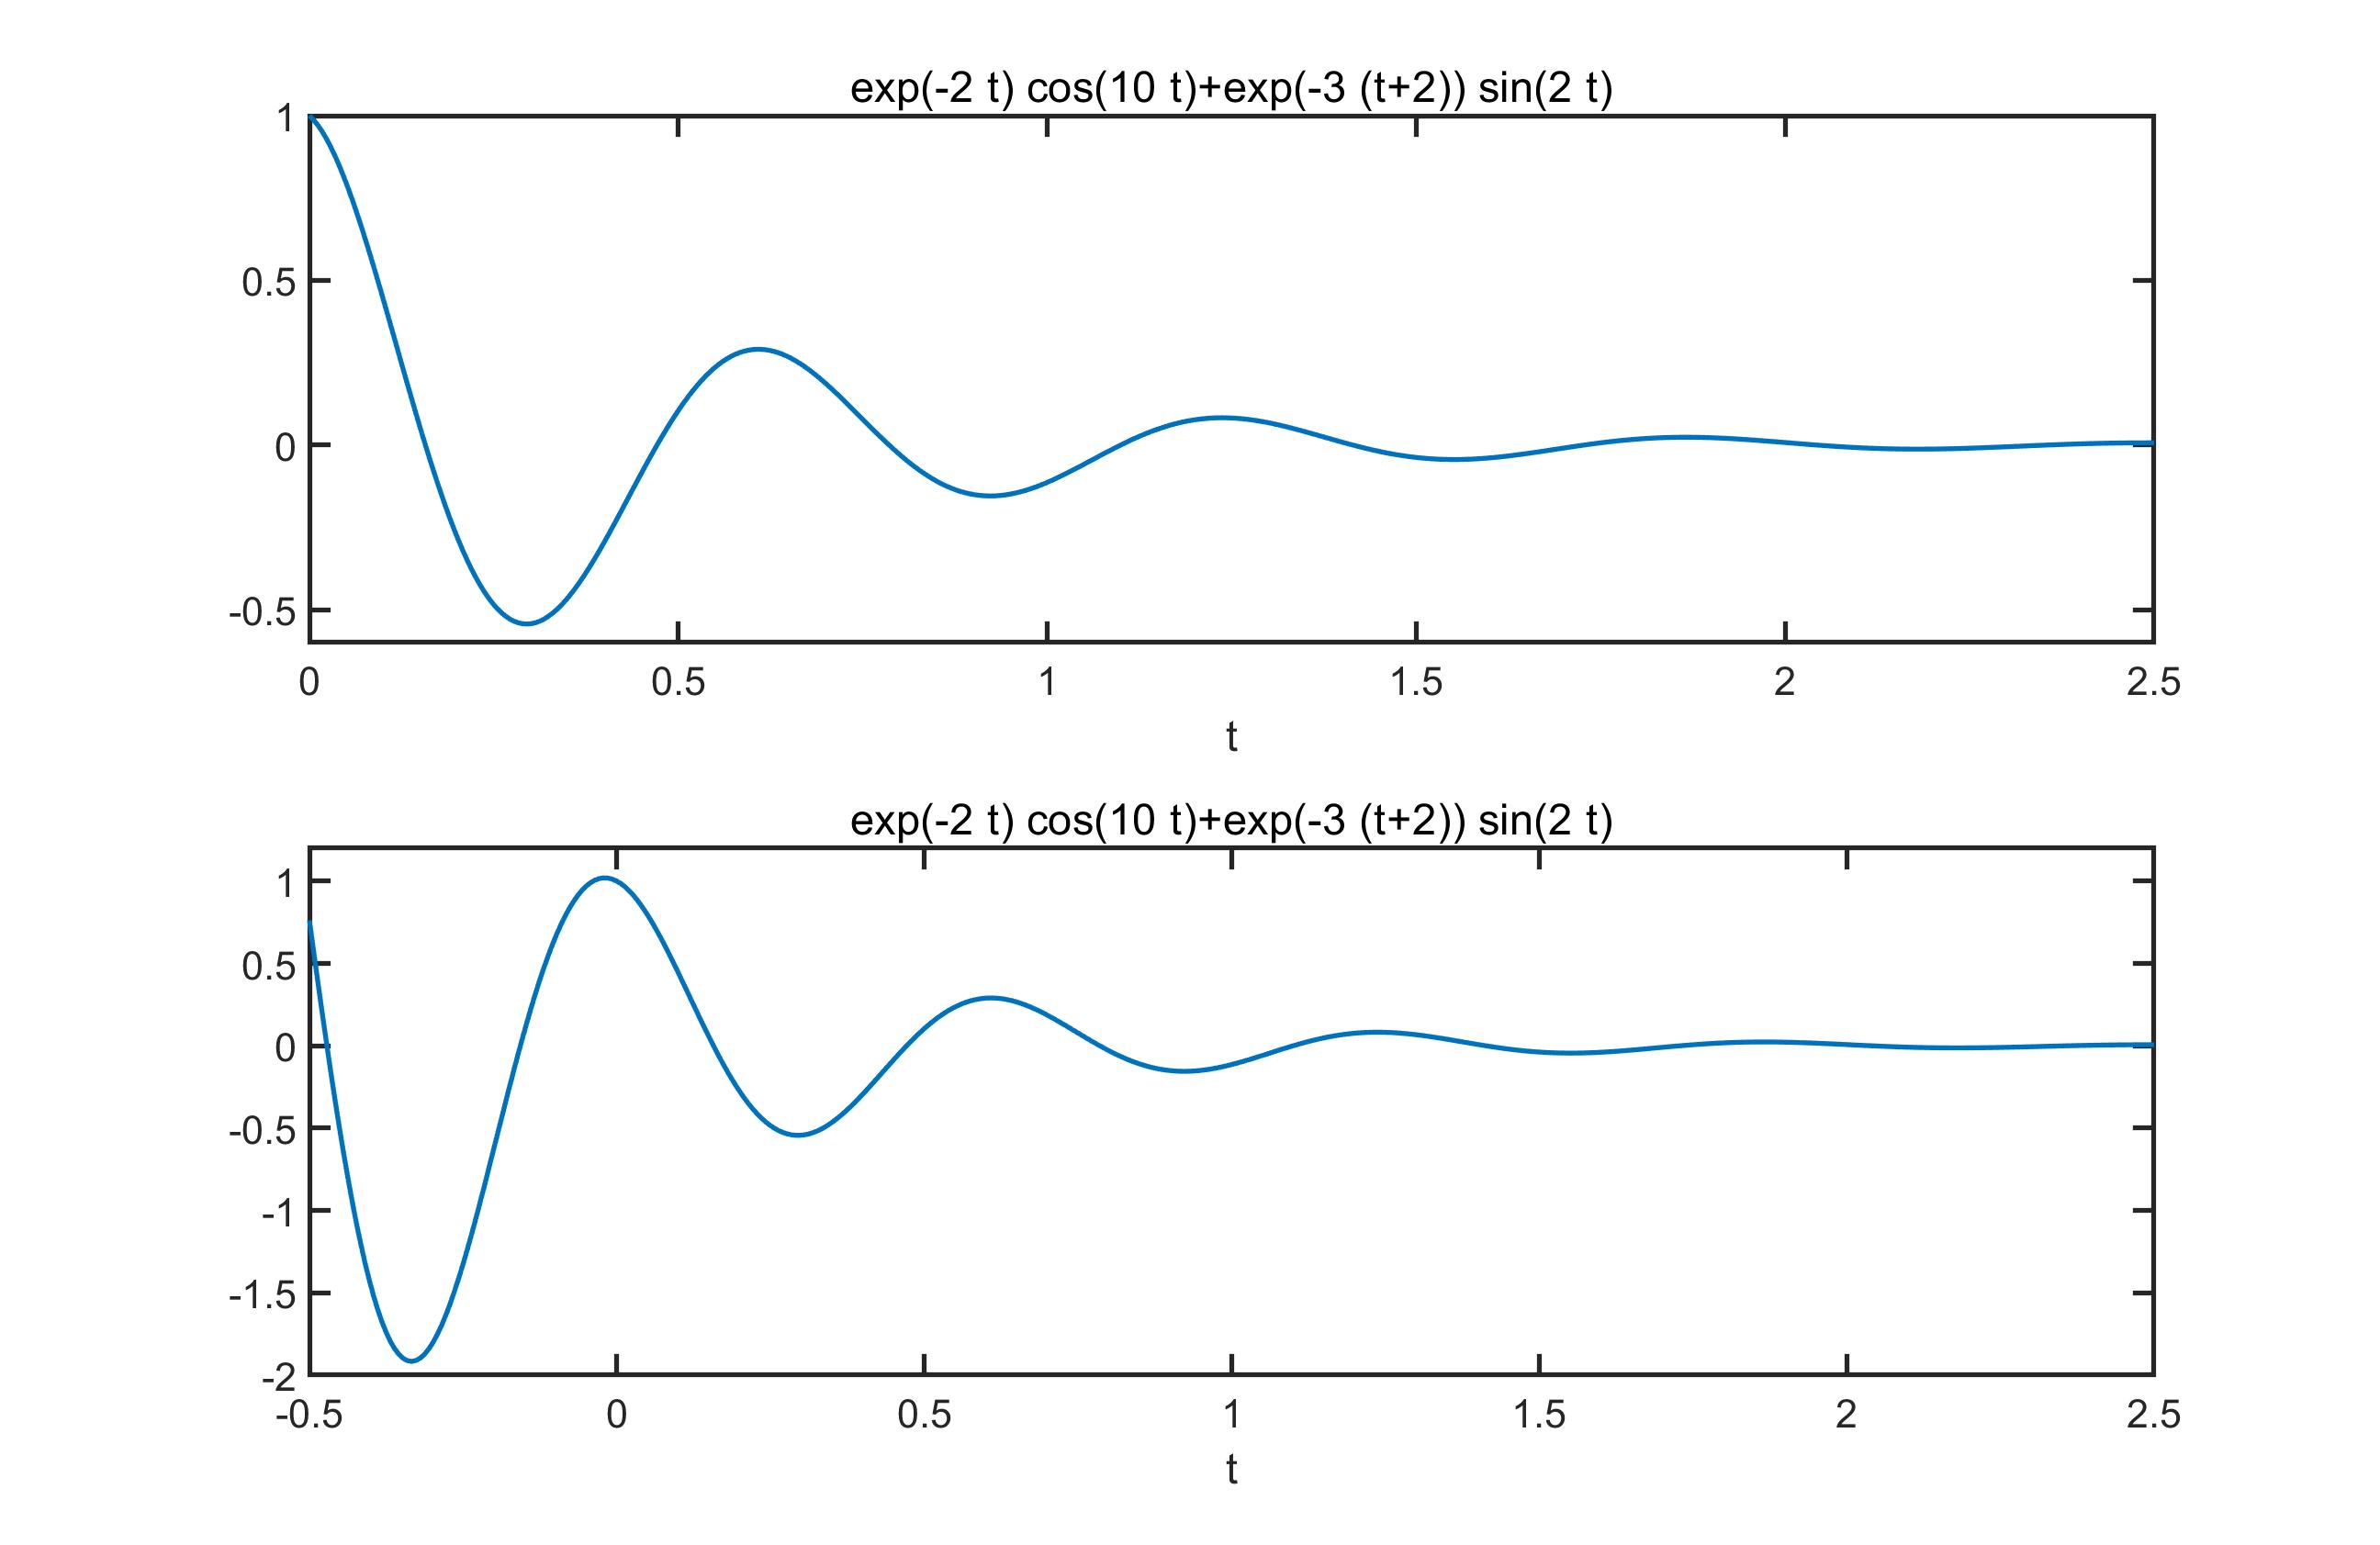
\includegraphics[width=.8\textwidth]{23}
			
	[t3\_1, f3\_1] =[0.9228, -0.1547] 初值t=1
	
	[t3\_2, f3\_2] =[0.2945, -0.5436] 初值t=.1
		\end{block}
		
	\end{columns}
\end{frame}
%---------------------------------------------------------------------- 
	% \subsection{利用梯度求解最优化问题}
\begin{frame}[fragile]{利用梯度求解最优化问题}
\textbf{思路:}引入目标函数梯度,加快计算速度,改进搜索精度,但影响计算速度。即设置 optimset.GradObj='on' 。
	
	\begin{example}[6-14]
求解Rosenbrock函数$f\left(x_{1}, x_{2}\right)=100\left(x_{2}-x_{1}^{2}\right)^{2}+\left(1-x_{1}\right)^{2}$无约束最优化问题。
	\end{example}
	
	\begin{block}{MATLAB代码:}
\begin{lstlisting}
ff4=@(x)100*(x(2)-x(1)^2)^2+(1-x(1))^2;
ff4_0 = optimset; ff4_0.Display='iter'; ff4_0.TolX = 1e-10; ff4_0.TolFun= 1e-20;
x4 = fminunc(ff4,[0; 0],ff4_0)
syms x1 x2
ff4_1=100*(x2-x1^2)^2+(1-x1)^2;
J = jacobian(ff4_1,[x1, x2]);
\end{lstlisting}
	\end{block}				
\end{frame}
%---------------------------------------------------------------------- 
\begin{frame}[fragile]{利用梯度求解最优化问题}
	\begin{columns}[T]
		\column{.65\textwidth}
	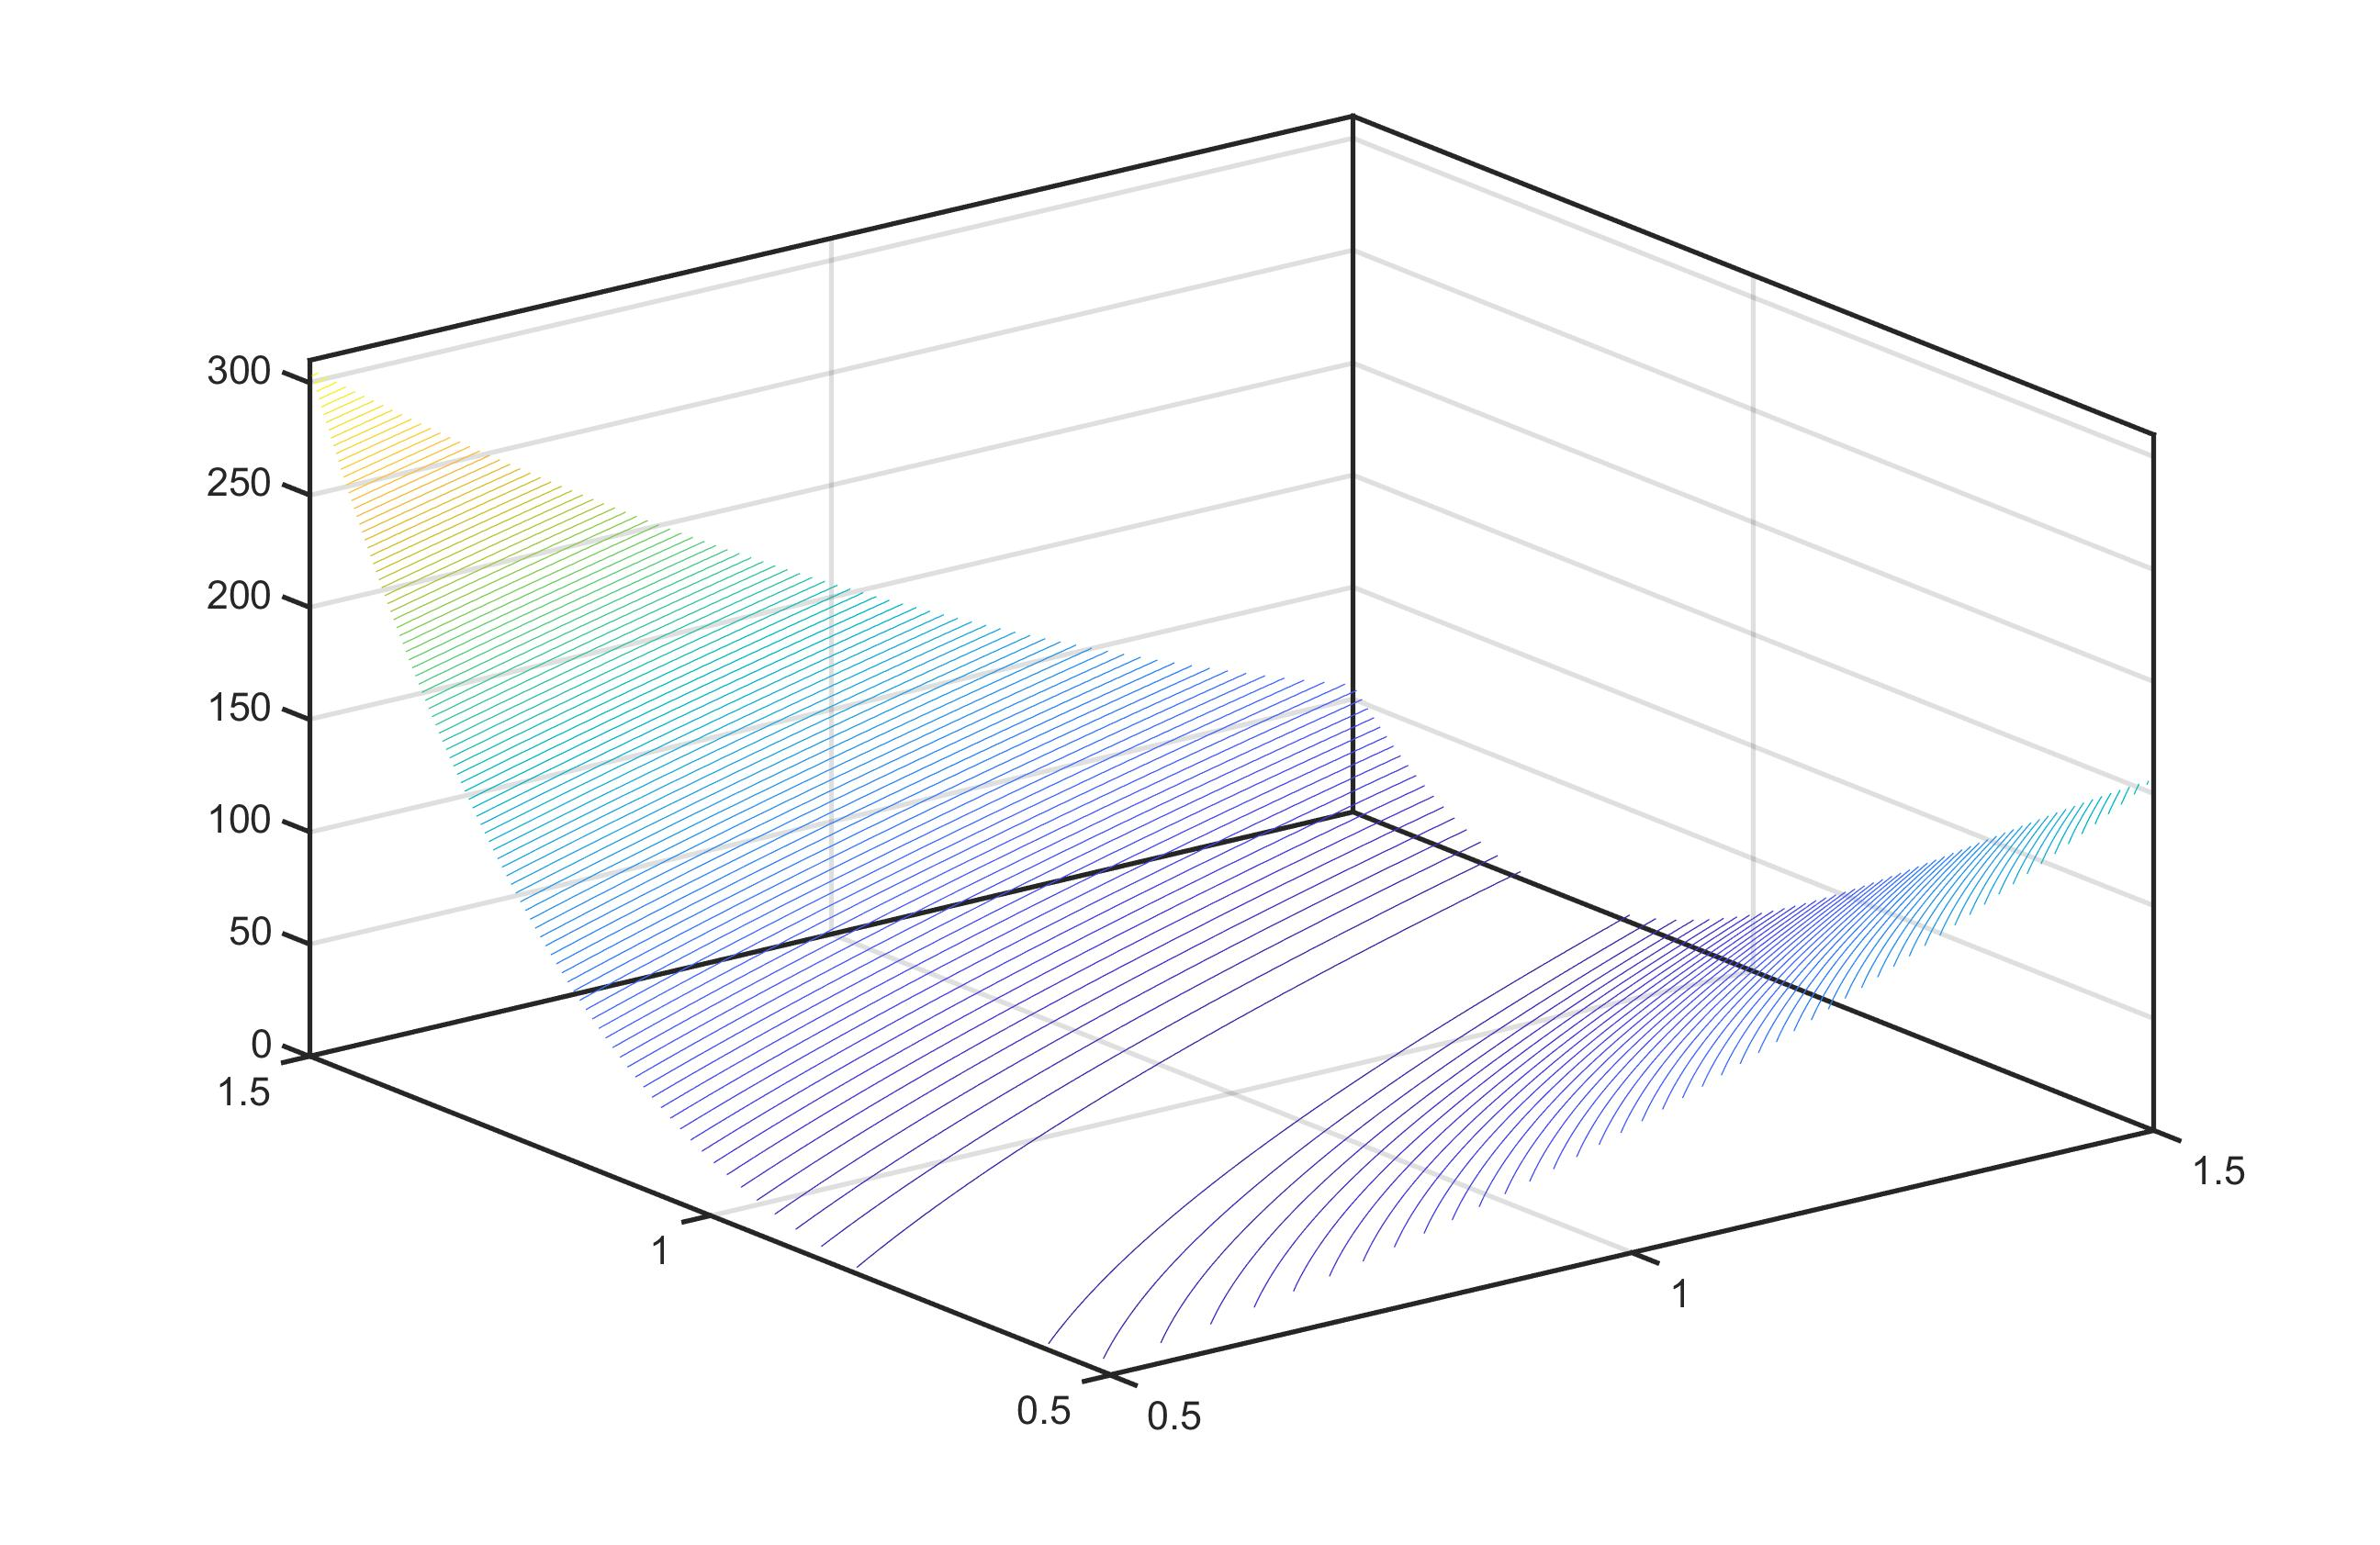
\includegraphics[width=\textwidth]{24}
		Rosenbrock函数,易知最小值(1,1)。

		\column{.4\textwidth}
\begin{block}{MATLAB代码(续):}
\begin{lstlisting}
ff4_0.GradObj='on';
x4_modi = fminunc(@ff4_modi,[0; 0],ff4_0)
function [y,Gy] = ff4_modi(x)
y = 100*(x(2)-x(1)^2)^2+(1-x(1))^2;
Gy = [2*x(1) - 400*x(1)*(- x(1)^2 + x(2)) - 2; - 200*x(1)^2 + 200*x(2)];
end
\end{lstlisting}
\end{block}	
	\end{columns}

\end{frame}
%---------------------------------------------------------------------- 
\begin{frame}[fragile]{利用梯度求解最优化问题}

\begin{lstlisting}                                            
Iteration  Func-count       f(x)        Step-size      First-order optimality
0           3                1                             2
1          12         0.771192      0.0817341           5.34  
......
20          81      1.94742e-11              1       1.06e-06
x4 = (1.0000,1.0000)
                   
Iteration  Func-count       f(x)        Step-size      First-order optimality
0           1                1                             2
1           4         0.771191      0.0817342           5.34  
......
22          29      1.16799e-23              1       1.26e-10
23          30      2.04561e-28              1       2.41e-13
x4_modi = (1.0000,1.0000)
\end{lstlisting}

\textbf{注:}实际情况常见带变量边界约束的最优化问题,如$\min\limits_{\mathbf{x}\ s.t.\ \mathbf{x_m} \leqslant \mathbf{x} \leqslant \mathbf{x_M}}$,可以调用fminsearchbnd()函数。

\end{frame}

%---------------------------------------------------------------------- 
\section{有约束最优化问题的计算机求解}
	% \subsection{约束条件与可行解区域}
		\begin{frame}[fragile]{约束条件与可行解区域}
			\textbf{有约束最优化问题提法:}$\min\limits_{\mathbf{x}\ s.t.\ \mathrm{G}(\mathbf{x}) \leqslant \mathbf{0}} f(\mathbf{x})$。满足$\mathrm{G}(\mathbf{x}) \leqslant \mathbf{0}$的范围称为可行解区域(feasible region)。
			
		\begin{columns}[T]
	\column{.5\textwidth}
				
		\begin{example}[6-15]
			二元最优化问题$
			\begin{array}{l}
			\max \quad \left(-x_{1}^{2}-x_{2}\right)\\
			\left\{\begin{array}{l}
			9 \geqslant x_{1}^{2}+x_{2}^{2} \\
			x_{1}+x_{2} \leqslant 1
			\end{array}\right.
			\end{array}
			$
		\end{example}
				
	\begin{block}{MATLAB代码:}
\begin{lstlisting}
syms x1 x2
[x1,x2]=meshgrid(-3:.1:3);
z = -x1.^2 - x2;
i = find(x1.^2 + x2.^2 > 9);  z(i) = NaN;
i = find(x1 + x2 > 1);  z(i) = NaN;
surf(x1,x2,z)
\end{lstlisting}
	\end{block}	
				
	\column{.55\textwidth}
				
	\begin{block}{输出:}
\centering
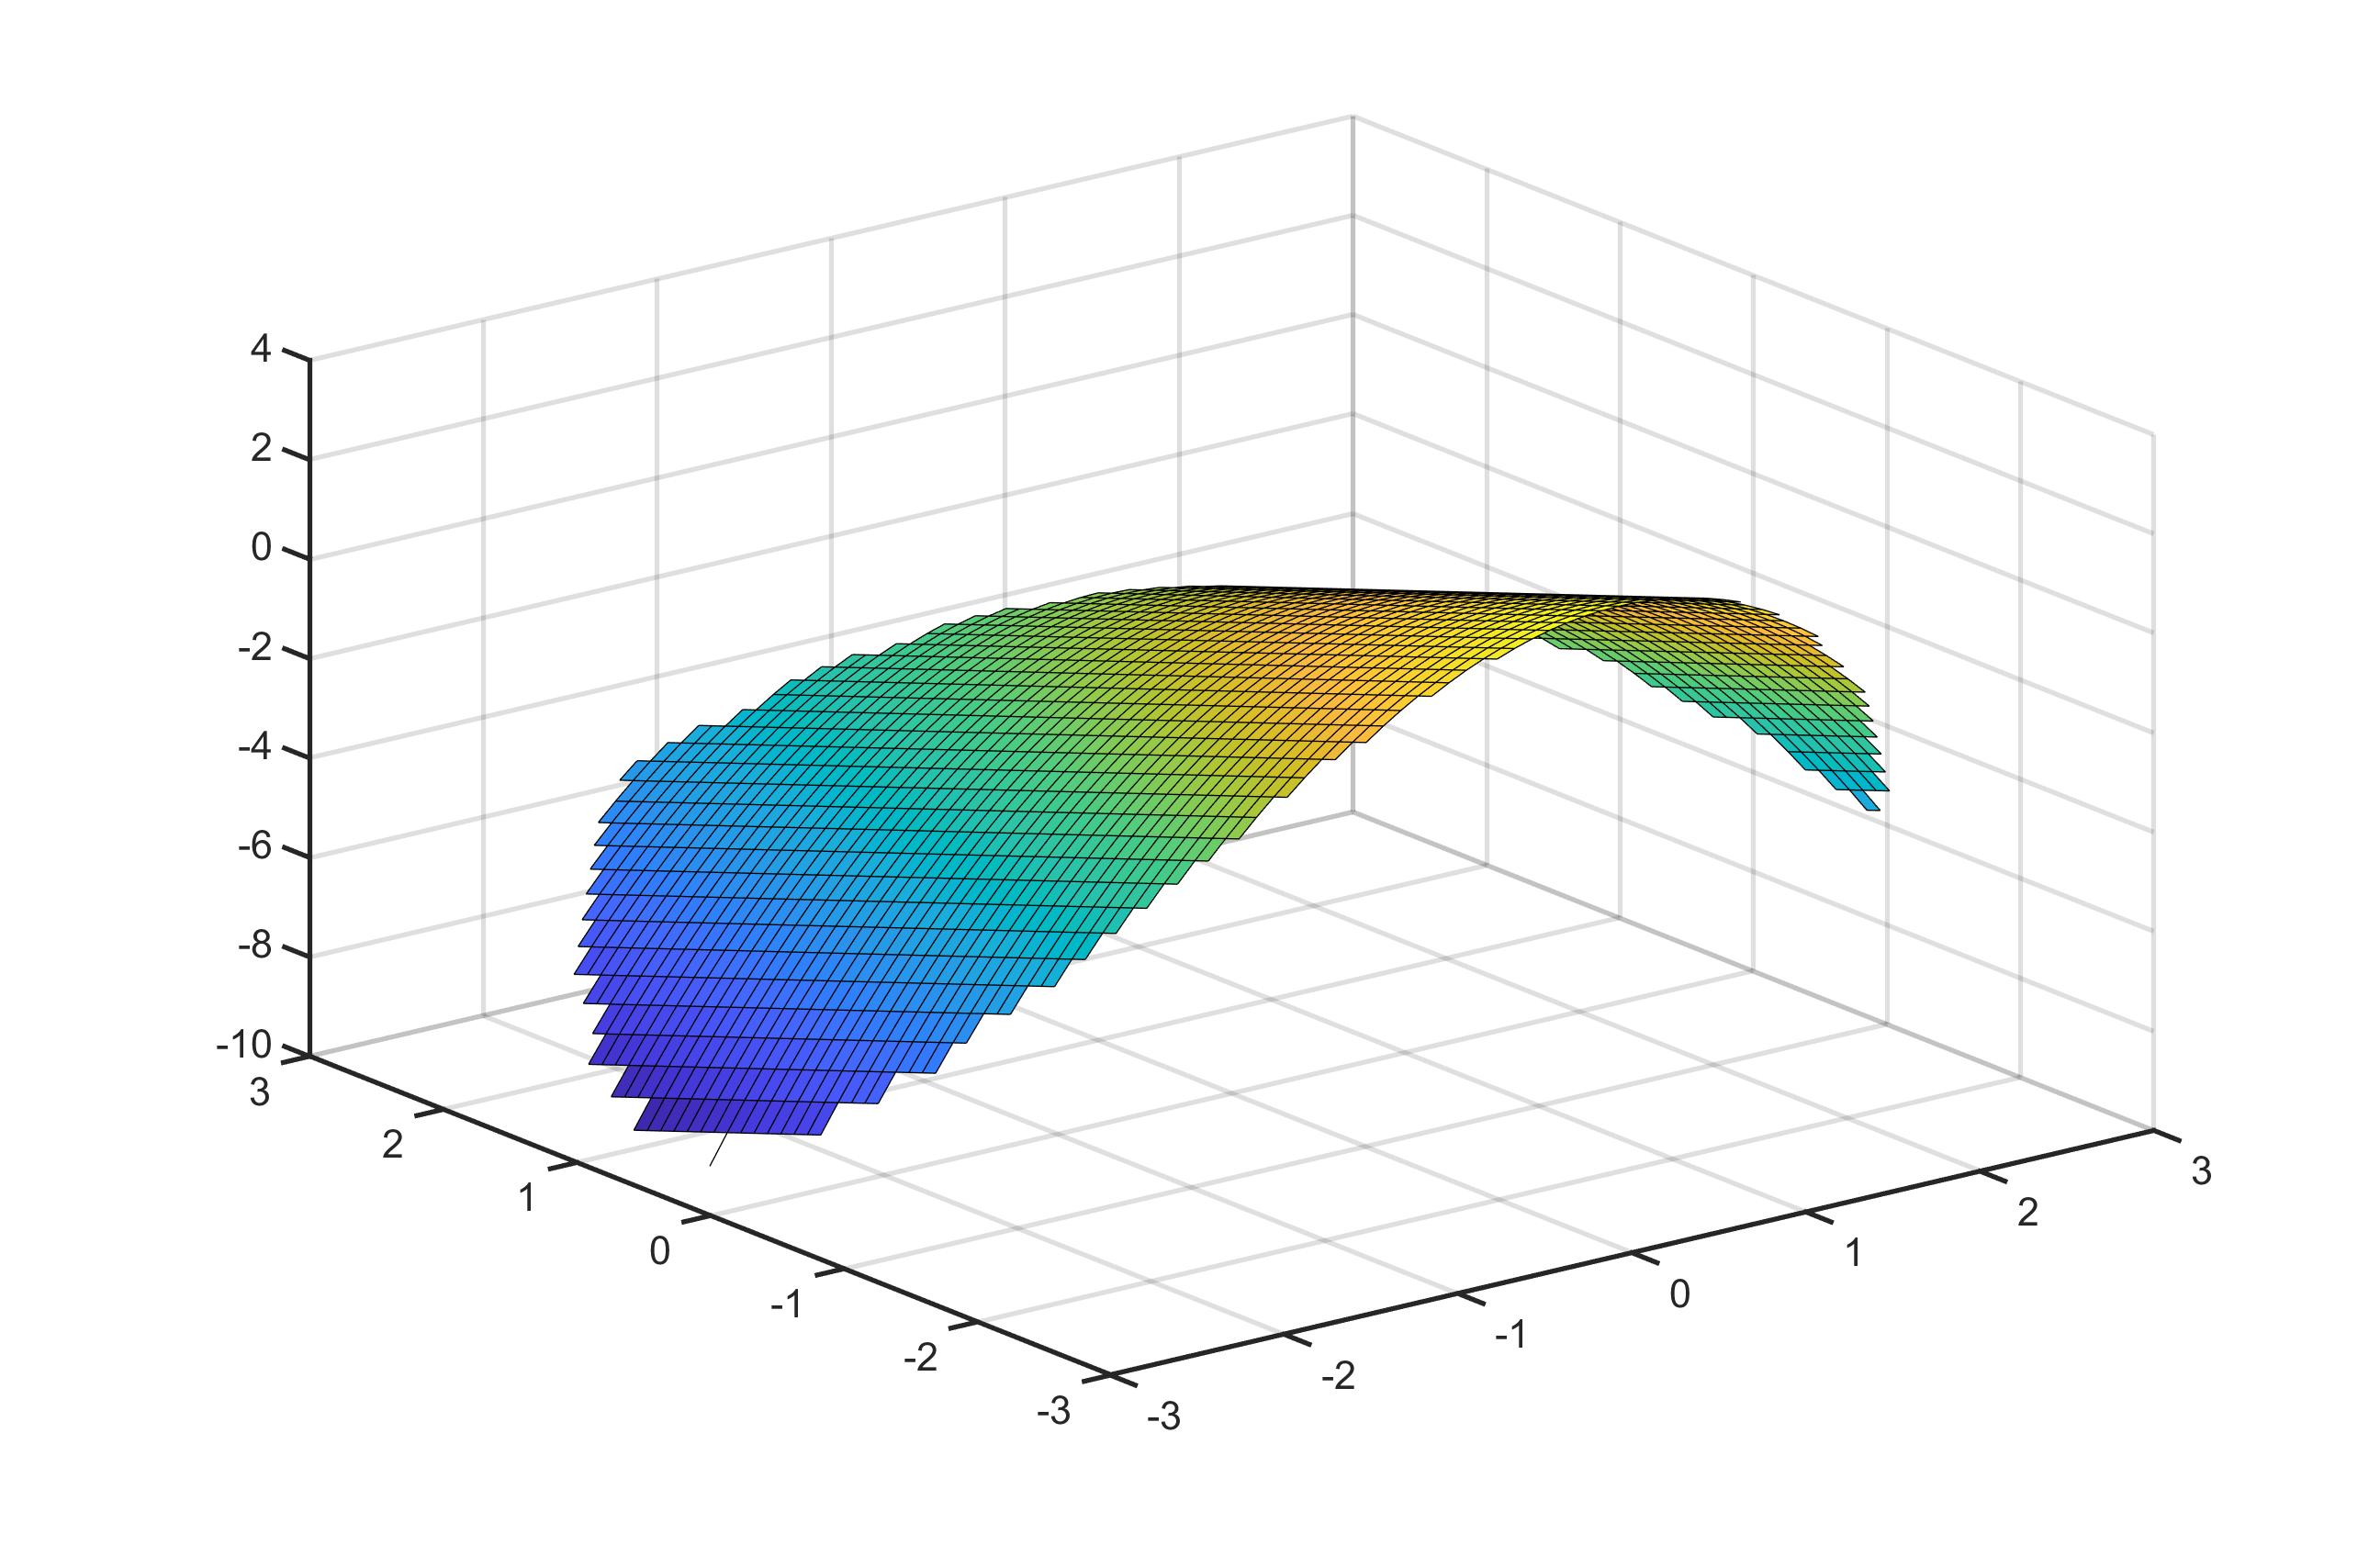
\includegraphics[width=\textwidth]{31}

max(z(:)) = 3,在(-3,0)处。
	\end{block}
		\end{columns}			
\end{frame}
%---------------------------------------------------------------------- 
	% \subsection{线性规划问题的计算机求解}
\begin{frame}[fragile]{线性规划问题的计算机求解}
	\textbf{线性规划问题提法:}$
	\begin{array}{l}
	\min \quad \mathbf{f}^T \mathbf{x}\\
	\mathbf{x} \text { s.t. }\left\{\begin{array}{l}
	\mathbf{A} \mathbf{x} \leqslant \mathbf{B} \\
	\mathbf{A}_{\mathrm{eq}} \mathbf{x}=\mathbf{B}_{\mathrm{eq}} \\
	\mathbf{x}_{m} \leqslant \mathbf{x} \leqslant \mathbf{x}_{M}
	\end{array}\right.
	\end{array}$,
	
	线性不等式约束:$\mathbf{A} \mathbf{x} \leqslant \mathbf{B}$,线性等式约束:$\mathbf{A}_{\mathrm{eq}} \mathbf{x}=\mathbf{B}_{\mathrm{eq}}$,上界变量$\mathbf{x}_{M}$,下界变量$\mathbf{x}_{m}$。
	
	\begin{block}{linprog()函数调用:}
\begin{lstlisting}
[x,f_opt,flag,c] = linprog(f, A, B, A_eq, B_eq, x_m, x_M, x_0, OPT, p1, p2,...)
\end{lstlisting}
	\end{block}	
	
\end{frame}
%---------------------------------------------------------------------- 

\begin{frame}[t,fragile]{线性规划问题的计算机求解}

\begin{example}[6-17]
	$\begin{array}{l}
	\min \quad \left(-2 x_{1}-x_{2}-4 x_{3}-3 x_{4}-x_{5}\right)\\
	\mathbf{x} \text { s.t. }\left\{\begin{array}{l}
	2 x_{2}+x_{3}+4 x_{4}+2 x_{5} \leqslant 54 \\
	3 x_{1}+4 x_{2}+5 x_{3}-x_{4}-x_{5} \leqslant 62 \\
	x_{1}, x_{2} \geqslant 0,, x_{3} \geqslant 3.32, x_{4} \geqslant 0.678, x_{5} \geqslant 2.57
	\end{array}\right.
	\end{array}
	$
\end{example}

	\begin{columns}[T]
		\column{.5\textwidth}
			
	\begin{block}{MATLAB代码:}
\begin{lstlisting}
f = [-2;-1;-4;-3;-1]; A = [0 2 1 4 2; 3 4 5 -1 -1]; B = [54; 62];
Ae=[]; Be=[]; xm=[0 0 3.32 .678 2.57]; 
ff5_0 = optimset; ff5_0.LargeScale = 'off'; ff5_0.Display = 'iter';
ff5_0.TolX = 1e-15; ff5_0.TolFun = 1e-10; ff5_0.TolCon = 1e-9; 
[x, f_opt, key, c] = linprog(f, A, B, Ae, Be, xm, [], [], ff5_0)
\end{lstlisting}
	\end{block}	
			
		\column{.55\textwidth}
			
	\begin{block}{输出:}
\begin{lstlisting}
Iter = 2, Time = 0.013 ......

x =
19.7850
0
3.3200
11.3850
2.5700

f_opt = -89.5750
\end{lstlisting}
	\end{block}

	\end{columns}		

\end{frame}
%---------------------------------------------------------------------- 
	% \subsection{二次型规划的求解}
		\begin{frame}[fragile]{二次型规划的求解}
	\textbf{二次型规划问题提法:}$
\begin{array}{l}
\min \quad \left(\frac{1}{2} \mathbf{x}^{\mathrm{T}} \mathbf{H} \mathbf{x}+\mathbf{f}^{\mathrm{T}} \mathbf{x}\right)\\
\mathbf{x} \text { s.t. }\left\{\begin{array}{l}
\mathbf{A} \mathbf{x} \leqslant \mathbf{B} \\
\mathbf{A}_{\mathrm{eq}} \mathbf{x}=\mathbf{B}_{\mathrm{eq}} \\
\mathbf{x}_{m} \leqslant \mathbf{x} \leqslant \mathbf{x}_{M}
\end{array}\right.
\end{array}$

	\begin{block}{quadprog()函数调用:}
\begin{lstlisting}
[x,f_opt,flag,c]=quadprog(H,f,A,B,A_eq,B_eq,x_m,x_M,x_0,OPT,p1,p2,...)
\end{lstlisting}
	\end{block}	

\begin{example}[6-18]
	$\begin{array}{l}
	\min \quad \left[\left(x_{1}-1\right)^{2}+\left(x_{2},+2\right)^{2}+\left(x_{3}-3\right)^{2}+\left(x_{4}-4\right)^{2}\right]\\
	\mathbf{x} \text { s.t. }\left\{\begin{array}{l}
	x_{1}+x_{2}+x_{3}+x_{4} \leqslant 5 \\
	3 x_{1}+3 x_{2}+2 x_{3}+x_{4} \leq 10 \\
	x_{1}, x_{2}, x_{3}, x_{4} \geqslant 0
	\end{array}\right.
	\end{array}
	$
\end{example}

\begin{block}{输出:}
	\begin{lstlisting}
Iter = 5...... x =(0.0000,0.6667,1.6667,2.6667); f_opt =-23.6667\end{lstlisting}
\end{block}	
			
		\end{frame}
%---------------------------------------------------------------------- 
	% \subsection{一般非线性规划问题的求解}
\begin{frame}[fragile]{一般非线性规划问题的求解}
\textbf{一般非线性规划问题提法}$
\begin{array}{l}
	\min \quad f(\mathbf{x})\\
	\mathbf{x} \text { s.t. }\left\{\begin{array}{ll}
		\mathbf{A} \mathbf{x} \leqslant \mathbf{B} &, \mathbf{A}_{\mathrm{eq}} \mathbf{x}=\mathbf{B}_{\mathrm{eq}} \\
		\mathbf{x}_{m} \leqslant \mathbf{x} \leqslant \mathbf{x}_{M} &,\mathbf{C}(\mathbf{x}) \leqslant 0 \\
		\mathbf{C}_{eq}(\mathbf{x})= 0 &.
	\end{array}\right.
\end{array}$
	\begin{block}{fmincon()函数调用:}
\begin{lstlisting}
[x,f_opt,flag,c]=fmincon(F,x0,A,B,A_eq,B_eq,x_m,x_M,CF,OPT,p1,p2,...)
%全局最优解尝试,则调fmincon_global()函数,规则同上。
\end{lstlisting}
	\end{block}

\begin{example}[6-19]
$\begin{array}{l}
\min \quad \left[1000-x_{1}^{2}-2 x_{2}^{2}-x_{3}^{2}-x_{1} x_{2}-x_{1} x_{3}\right]\\
\mathbf{x} \text { s.t. }\left\{\begin{array}{l}
x_{1}^{2}+x_{2}^{2}+x_{3}^{2}-25=0 \\
8 x_{1}+14 x_{2}+7 x_{3}-56=0 \\
x_{1}, x_{2}, x_{3} \geqslant 0
\end{array}\right.
\end{array}
$
\end{example}
\end{frame}
%---------------------------------------------------------------------- 
\begin{frame}[fragile]{一般非线性规划问题的求解}
	\begin{block}{MATLAB代码}
\begin{lstlisting}
ff8_0 = optimset; ff8_0.LargeScale = 'off'; ff8_0.Display = 'iter';
ff8_0.TolX = 1e-15; ff8_0.TolFun = 1e-30; ff8_0.TolCon = 1e-20; 
x0=ones(3,1); xm=zeros(3,1); xM=[]; A=[]; B=[]; Aeq=[]; Beq=[];
[x,f_opt,flag,c] = fmincon(@opt_fun1, x0, A, B, Aeq, Beq, xm, xM, @opt_con1, ff8_0)
\end{lstlisting}		
	\end{block}	
	
	\begin{block}{输出}
\begin{lstlisting}
x =
3.5121
0.2170
3.5522

f_opt =
961.7152

iterations: 16
\end{lstlisting}		
	\end{block}	

\end{frame}
%----------------------------------------------------------------------	
% \section{其他}
	% \subsection{应用实例}
%		\begin{frame}[allowframebreaks]{应用实例}
%		
%		\end{frame}
%---------------------------------------------------------------------- 	
	% \subsection{学习心得}
		\begin{frame}[allowframebreaks]{学习心得}
	\textbf{一}\quad 这是本系统具体的书,可以了解,明白MATLAB能解决的问题,有实际需要时再详细翻阅。
	
	\textbf{二}\quad MATLAB集成很多科学计算算法,也方便调用。我联想到了FFTW、LAPACK等,让用户避免重复造轮子。
	但我认为需要对算法有些了解,定性明白它的长处和不足。
		\end{frame}

% lzr

\section{混合整数规划问题的计算机求解}
\begin{frame}[allowframebreaks]
  \frametitle{整数规划}
  
  在很多应用领域中,最优化问题需要额外要求全部或部分自变量取整数,这类问题又称为整数规划.
  \begin{figure}
  \centering
  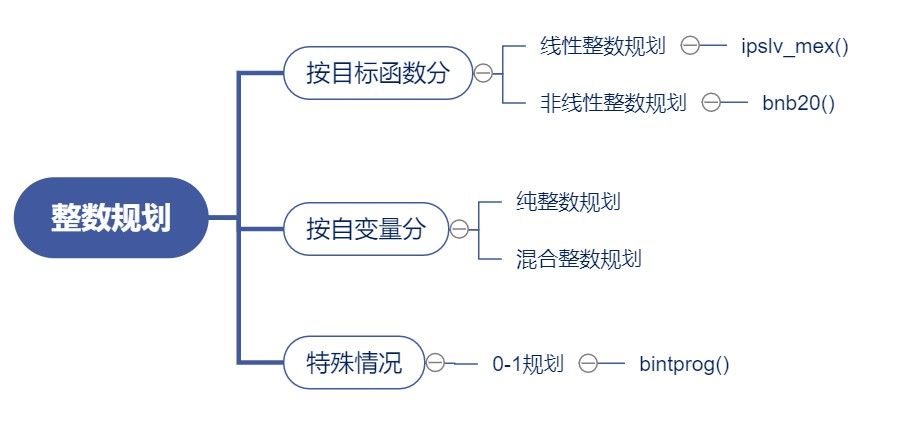
\includegraphics[width=0.88\textwidth]{zsgh.jpg}
  \caption{整数规划的划分}
  \end{figure}
  \end{frame}
  
  \begin{frame}[allowframebreaks]
  \frametitle{整数线性规划问题的求解}
  
  \begin{equation}
  \begin{array}{c}
  \min f^{T} x \\
  x \in Z \text { s.t.}\left\{\begin{array}{c}
  A x \leq B \\
  A_{e q} x=B_{e q} \\
  x_{m} \leq x \leq x_{M}
  \end{array}\right.
  \end{array}
  \end{equation}
  
  之前MATLAB没有提供整数线性规划的函数,常用有代表性的Michel Berkelaar等人开发的lpslv包.
  \begin{equation}
  [x, h o w]=i p s l v_{-} \operatorname{mex}\left(A, B, f, \text {intlist}, x_{m}, x_{M}, \text {ctype}\right)
  \end{equation}
  \end{frame}
  
  \begin{frame}[allowframebreaks]
  \frametitle{一般非线性整数规划问题与求解}
  
  实际应用中经常需要求解非线性整数规划或混合规划问题,常用求解函数是基于分枝定界算法编写的bnb20函数.
  \begin{equation}
  [e r r, f, x]=b n b 20\left(f u n, x_{0}, \text { intlist }, x_{m}, x_{M}, A, B, A_{e q}, B_{e q}\right)
  \end{equation}
  该函数主要调用的是最优化工具箱函数.
  \end{frame}
  
  \begin{frame}[allowframebreaks]
  \frametitle{0-1规划问题求解}
  
  MATLAB提供了用来求解0-1线性规划问题的函数bintprog,但不能直接求解非线性0-1规划问题.
  \begin{equation}
  x=\operatorname{bintprog}\left(f, A, B, A_{e q}, B_{e q}\right)
  \end{equation}
  免费的MAILAB函数求解非线性混合整数规划的功能不是很强大,基于MATLAB的商业软件TOMLAB更复杂,但功能也更加全面且出色.
  \end{frame}
  
  \begin{frame}[allowframebreaks]
  \frametitle{应用举例}
  
  MATLAB后续版本中更新了MILP函数,可以求解混合线性整数规划问题.
  \begin{equation}
  x=\operatorname{intlinprog}\left(f, \text {intcon,} A, B, A_{e q}, B_{e q}, x_{m}, x_{M}\right)
  \end{equation}
  以解下面的优化问题为例
  \begin{equation}
  \begin{array}{c}
  \min \left(-2 x_{1}-x_{2}-4 x_{3}-3 x_{4}-x_{5}\right) \\
  2 x_{2}+x_{3}+4 x_{4}+2 x_{5} \leq 54 \\
  3 x_{1}+4 x_{2}+5 x_{3}-x_{4}-x_{5} \leq 62 \\
  x_{1} \geq 0, x_{2} \geq 0, x_{3} \geq 3.32, x_{4} \geq 0.678, x_{5} \geq 2.57
  \end{array}
  \end{equation}
  \end{frame}
  
  \begin{frame}[allowframebreaks]
  \frametitle{结果}
  
  \begin{equation}
  \begin{array}{c}
  \min \left(-2 x_{1}-x_{2}-4 x_{3}-3 x_{4}-x_{5}\right) \\
  2 x_{2}+x_{3}+4 x_{4}+2 x_{5} \leq 54 \\
  3 x_{1}+4 x_{2}+5 x_{3}-x_{4}-x_{5} \leq 62 \\
  x_{1} \geq 0, x_{2} \geq 0, x_{3} \geq 3.32, x_{4} \geq 0.678, x_{5} \geq 2.57
  \end{array}
  \end{equation}
  \begin{figure}
  \centering
  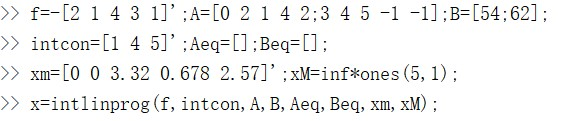
\includegraphics[width=0.88\textwidth]{test1.jpg}
  \caption{参数输入}
  \end{figure}
  
  \begin{figure}
  \centering
  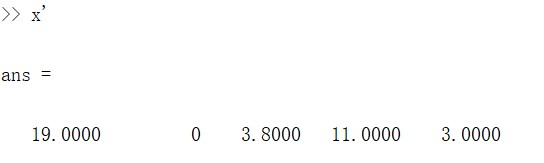
\includegraphics[width=0.72\textwidth]{ans1.jpg}
  \caption{算例结果}
  \end{figure}
  时间客观上是连续的,但社会时间是离散的,整数规划相较于连续优化问题,看似是简化了条件,实际的解决难度却并没有降低,并且其在交通、能源等诸多实际领域中具有更高的应用价值。但是也不能否定了连续优化的作用,科学的本质便是从简到难,先把简单问题研究透彻,再把复杂问题简化为求解一个个简单的问题.
  \end{frame}

% zzm
\section{线性矩阵不等式问题求解}

\begin{frame}[allowframebreaks]{6.5.1线性矩阵不等式}
  线性矩阵不等式具有一般的描述形式
  \\$\boldsymbol{F}\left ( x\right )=\boldsymbol{F}_{0}+x_{1}\boldsymbol{F}_{1}+\cdots +x_{m}\boldsymbol{F}_{m}< 0$
  \\其中:$\boldsymbol{x}=\left [ x_{1},x_{2},\cdots x_{m},\right ]^{T}$ ,为多项式向量,$\boldsymbol{F}_{1}$为实对称矩阵或者复Hermite矩阵。
  
  矩阵小于零表示矩阵负定。有$\boldsymbol{x}$解集为凸集,即:
  \\$ \boldsymbol{F}\left [ \alpha \boldsymbol{x}_{1}+\left ( 1-\alpha \right )\boldsymbol{x}_{2}\right ]=\alpha \boldsymbol{F}\left ( \boldsymbol{x}_{1} \right ) +\left ( 1-\alpha \right )\boldsymbol{F}\left ( \boldsymbol{x}_{2} \right )< 0$
  \\其中$0< \alpha < 1$,该解称为可行解。
  
  
  \end{frame}
  
  \begin{frame}[allowframebreaks]{6.5.1线性矩阵不等式}
  若有$\boldsymbol{F}_{1}\left ( x\right )< 0$与$\boldsymbol{F}_{2}\left ( x\right )< 0$则
  
  \[\begin{bmatrix}
  \boldsymbol{F}_{1}\left ( x\right ) & 0\\ 
  0 & \boldsymbol{F}_{2}\left ( x\right )
  \end{bmatrix}< 0\]
  同理有系列$\boldsymbol{F}_{i}\left ( x\right )< 0$, $i=1,2,...,k$
  可有\[\boldsymbol{F}\left ( x\right )=\begin{bmatrix}
  \boldsymbol{F}_{1}\left ( x\right ) &  &  & \\ 
  &  \boldsymbol{F}_{2}\left ( x\right ) & & \\ 
  &  & \cdots & \\ 
  &  &  & \boldsymbol{F}_{k}\left ( x\right )
  \end{bmatrix}< 0\]
  \end{frame}
  
  \begin{frame}[allowframebreaks]{6.5.2Lyapunov不等式}
  若给定正定矩阵$\boldsymbol{Q}$,有Lyapunov方程:
  \\$\boldsymbol{A}^{T}\boldsymbol{X}+\boldsymbol{X}\boldsymbol{A}=-\boldsymbol{Q}$
  \\若存在正定的解$\boldsymbol{X}$则该系统稳定。上述问题很自然地表示成对Lyapunov不等式的求解\[\boldsymbol{A}^{T}\boldsymbol{X}+\boldsymbol{X}\boldsymbol{A}< 0\]
  $\boldsymbol{X}$是对称矩阵,可以用一个$n\left ( n+1\right )/2$哥元素组成的向量$\boldsymbol{x}$描述:
  \[x_{i-j+1+\left ( 2n-j+2\right )\left ( j-1\right )/2}=X_{i,j}\]
  其中$j=1,..,n$而$i=j,...,n$。
  \end{frame}
  
  \begin{frame}[allowframebreaks]{6.5.2Lyapunov不等式}
  接着便可以将\[\boldsymbol{A}^{T}\boldsymbol{X}+\boldsymbol{X}\boldsymbol{A}< 0\]
  转化为\[\begin{bmatrix}
  \boldsymbol{F}_{1} &  &  & \\ 
  & \boldsymbol{F}_{2} &  & \\ 
  &  & \cdots  & \\ 
  &  &  & \boldsymbol{F}_{\frac{n\left ( n+1\right )}{2}}
  \end{bmatrix}\cdot \boldsymbol{x}=\boldsymbol{F}\left ( \boldsymbol{x}\right )< 0 \]
  matlab中用F
  \end{frame}
  
  \begin{frame}[allowframebreaks]{6.5.2一般代数Riccati不等式}
  我们知道若\[\boldsymbol{F}\left ( \boldsymbol{x}\right )=\begin{bmatrix}
  \boldsymbol{F}_{11}\left ( \boldsymbol{x}\right ) & \boldsymbol{F}_{12}\left ( \boldsymbol{x}\right )\\ 
  \boldsymbol{F}_{21}\left ( \boldsymbol{x}\right ) & \boldsymbol{F}_{22}\left ( \boldsymbol{x}\right )
  \end{bmatrix}\]是负定的,则有一下三个等价表达:
  \[\boldsymbol{F}\left ( \boldsymbol{x}\right )< 0\]\[\boldsymbol{F}_{11}\left ( \boldsymbol{x}\right )< 0,\boldsymbol{F}_{22}\left ( \boldsymbol{x}\right )-\boldsymbol{F}_{21}\left ( \boldsymbol{x}\right )\boldsymbol{F}_{11}^{-1}\left ( \boldsymbol{x}\right )\boldsymbol{F}_{12}\left ( \boldsymbol{x}\right )< 0\]\[\boldsymbol{F}_{22}\left ( \boldsymbol{x}\right )< 0,\boldsymbol{F}_{11}\left ( \boldsymbol{x}\right )-\boldsymbol{F}_{12}\left ( \boldsymbol{x}\right )\boldsymbol{F}_{22}^{-1}\left ( \boldsymbol{x}\right )\boldsymbol{F}_{21}\left ( \boldsymbol{x}\right )< 0\]
  \end{frame}
  
  \begin{frame}[allowframebreaks]{6.5.2一般代数Riccati不等式}
  对于更复杂的Riccati方程变换可以得到Riccati不等式
  \[\boldsymbol{A}^{T}\boldsymbol{X}+\boldsymbol{X}\boldsymbol{A}+\left ( \boldsymbol{X}\boldsymbol{B}-\boldsymbol{C}^{T}\right )\boldsymbol{R}^{-1}\left ( \boldsymbol{X}\boldsymbol{B}-\boldsymbol{C}^{T}\right )^{T}< 0\]
  对比
  \[\boldsymbol{F}_{22}\left ( \boldsymbol{x}\right )< 0,\boldsymbol{F}_{11}\left ( \boldsymbol{x}\right )-\boldsymbol{F}_{12}\left ( \boldsymbol{x}\right )\boldsymbol{F}_{22}^{-1}\left ( \boldsymbol{x}\right )\boldsymbol{F}_{21}\left ( \boldsymbol{x}\right )< 0\]
  可等价构建为
  \[\boldsymbol{X}> 0,\begin{bmatrix}
  \boldsymbol{A}^{T}\boldsymbol{X}+\boldsymbol{X}\boldsymbol{A} & \boldsymbol{XB}-\boldsymbol{C}^{T}\\ 
  \boldsymbol{B}^{T}\boldsymbol{X}-\boldsymbol{C}& -\boldsymbol{R}
  \end{bmatrix}< 0\]
  \end{frame}
  \begin{frame}[allowframebreaks]{6.5.3线性矩阵不等式问题分类}
  (1)可行性问题,即:
  \[\boldsymbol{F}\left ( \boldsymbol{x}\right )< 0\]
  存在解
  
  (2)线性目标函数最优化问题,即求:
  \\	\qquad \qquad\qquad\qquad\qquad\qquad min  
  $
  \boldsymbol{c}^{T}\boldsymbol{x}
  $
  \\\qquad\qquad\qquad\qquad\qquad
  $
  \boldsymbol{x}\;s.t.
  \boldsymbol{F}\left ( \boldsymbol{x}\right )< 0
  $
  
  (3)广义特征值最优化问题,即求:
  
    \qquad \qquad\qquad\qquad\qquad\qquad min 
  $
  \lambda 
  $
  \\\qquad\qquad\qquad\qquad
  $
  \lambda $ $\textbf{x}\;s.t.
  \left\{
  \begin{array}{ccc}
  \boldsymbol{A}\left ( \boldsymbol{x}\right )< \lambda \boldsymbol{B}\left ( \boldsymbol{x}\right ) \\
  \boldsymbol{B}\left ( \boldsymbol{x}\right )> 0\\
  \boldsymbol{C}\left ( \boldsymbol{x}\right )< 0 
  \end{array} 
  \right.
  $
  
  \end{frame}
  
  \begin{frame}[allowframebreaks]{6.5.4线性矩阵问题matlab求解}


	\begin{columns}[T]
		\column{.45\textwidth}
  
    考虑Riccati不等式
    \[\boldsymbol{A}^{T}\boldsymbol{X}+\boldsymbol{X}\boldsymbol{A}+\left ( \boldsymbol{X}\boldsymbol{B}\right )\boldsymbol{R}^{-1} \boldsymbol{B}^{T}\boldsymbol{X}+\boldsymbol{Q}< 0\]
    分块为\[\begin{bmatrix}
    \boldsymbol{A}^{T}\boldsymbol{X}+\boldsymbol{X}\boldsymbol{A}+\boldsymbol{Q} &\boldsymbol{X}\boldsymbol{B} \\ 
    \boldsymbol{B}^{T}\boldsymbol{X} & -\boldsymbol{R}
    \end{bmatrix}< 0\]
    
		\column{.45\textwidth}

    \begin{figure}[htp]
      \centering
      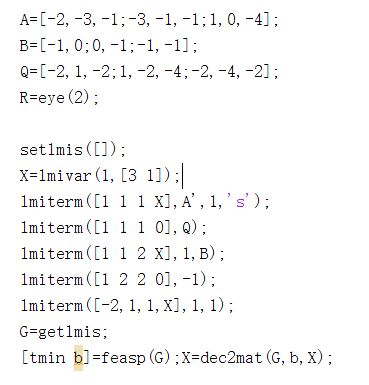
\includegraphics[width=0.9\textwidth]{51.jpeg}
      \caption{}
    \end{figure}
	\end{columns}


  
  \end{frame}
  
  \begin{frame}[allowframebreaks]{6.5.4线性矩阵问题matlab求解}
  
  带入:$\boldsymbol{A}=\begin{bmatrix}
  -2 & -3 & -1\\ 
  -3 & -1 & -1\\ 
  1 & 0 & -4
  \end{bmatrix}$
  
  $\boldsymbol{B}=\begin{bmatrix}
  -1 & 0 \\ 
  0 & -1\\ 
  -1 & -1
  \end{bmatrix}$
  $\boldsymbol{Q}=\begin{bmatrix}
  -2 & 1 & -2\\ 
  1 & -2 & -4\\ 
  -2 & -4 & -2
  \end{bmatrix}$
  $\boldsymbol{R}=\begin{bmatrix}
  1 & 0 \\ 
  0 & 1\\ 
  \end{bmatrix}$
  
  得到\[\boldsymbol{X}=\begin{bmatrix}
  0.9101 & 0.4641 & -0.2354\\ 
  0.4641 & 0.7893 & -0.0383\\ 
  -0.2354 & -0.0383 & 1.3616
  \end{bmatrix}\]
  
  
  \end{frame}
  
  \begin{frame}[allowframebreaks]{6.5.5基于Yalmip工具箱最优化求解方法}
    \begin{columns}[T]

  \column{.6\textwidth}
  
  YALMIP工具箱解决线性规划;
  \\	\qquad \qquad\qquad\qquad min \qquad 
  $
  6x_{1}-3x_{2}-5x_{3}-2x_{4}-9x_{5} 
  $
  \\\qquad\qquad\qquad
    $\textbf{x}\;s.t.
  \left\{
  \begin{array}{ccc}
  2x_{2}+x_{3}+4x_{4}+2x_{5} \leq 54 \\
  3x_{1}+4x_{2}+5x_{3}-x_{4}-x_{5} \leq 66\\
  x_{1}\geq 0,x_{2}\geq 2,x_{3}\geq3, x_{4}\geq 0.5,x_{5} \geq 2
  \end{array} 
  \right.
  $
  得到$x_{1}=22,x_{2}= 2,x_{3}=3, x_{4}= 0.5,x_{5} = 22.5$
  \\$
  6x_{1}-3x_{2}-5x_{3}-2x_{4}-9x_{5} =-356.5
  $
  
  
  \column{.4\textwidth}

  \begin{figure}[htp]
    \centering
    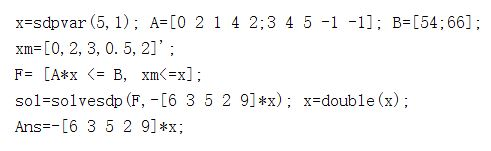
\includegraphics[width=1.1\textwidth]{52.jpeg}
    \caption{}
  \end{figure}
\end{columns}

  \end{frame}

% dhx
\section{多目标优化模型}

\begin{frame}[allowframebreaks]{多目标优化模型}
  例6-58  设商店有糖果A1,A2,A3,价格分别为4,2.8,2.4元/kg。要求购买不超过20元,总重不超过6kg。A1+A2总重不少于3kg,如何购买?
  \\应该设立两个目标函数,一个是花钱最少,一个是重量最总,其他条件可以认为是约束条件。假设购买三种糖果的重量分别为x1, x2, x3kg,这时目标函数分别为
  \\花钱:$f_1(x) = 4x_1+2.8x_2+2.4x_3 \rightarrow min$
  \\重量:$f_2(x) = x_1+x_2+x_3 \rightarrow \max$ 
  那么模型该如何设立呢?
  \end{frame}
  \begin{frame}[allowframebreaks]{多目标优化模型}
    \qquad min\qquad \qquad \qquad \qquad \qquad
    $
    \left[
    \begin{array}{ccc}
    4x_1+2.8x_2+2.4x_3	\\
    x_1+x_2+x_3	
    \end{array} 
    \right]
    $
    \\
    $
    \bm{x}\;s.t.
    \left\{
    \begin{array}{ccc}
    4x_1+2.8x_2+2.4x_3\leq20\\
    x_1+x_2+x_3\geq6\\
    x_1+x_2\geq3 \\
    x_1,x_2,x_3\geq0 
    \end{array} 
    \right.
    $
    \\从这之中我们可以得出多目标优化模型的一般表示形式:
    $$ \qquad \ J\qquad = \qquad \min\qquad \bm{F(x)}$$
    $$ \bm{x}\ s.t.  \bm{G(x)}\leq0$$
    其中,$\bm{F(x)} = [f_1(\bm{x}),f_2(\bm{x}),f_3(\bm{x}),\cdot \cdot \cdot,f_p(\bm{x})]^T$
  \end{frame}

\begin{frame}[allowframebreaks]{多目标问题转化为单目标问题求解}
  那么如何解这类问题呢?
  
  下面介绍三种转换方法:
  \begin{enumerate}
    \item 线性加权变换及求解
    \item 线性规划问题的最佳妥协解
    \item 线性规划问题的最小二乘解
  \end{enumerate}

\end{frame}

\begin{frame}[allowframebreaks]{(1)线性加权变换及求解}
    根据两个指标的侧重情况引入加权,目标函数改写为:
    $$f(\bm{x}) = w_1f_1(\bm{x})+ w_2f_2(\bm{x})+ w_3f_3(\bm{x})+\cdot \cdot \cdot+w_pf_p(\bm{x})$$
    其中,$w_1+w_2+\cdot \cdot \cdot+w_p=1$, $0\leq w_1,w_2,\cdot \cdot \cdot,w_p\leq 1$.	
    \\则例6-58就可以改写成下面的线性规划系数\\
    \qquad min\qquad \qquad \qquad \qquad \qquad
    $(w_1[4,2.8,2.4]-w_2[1,1,1])\bm{x}$
    \\
    $
    \bm{x}\;s.t.
    \left\{
    \begin{array}{ccc}
      4x_1+2.8x_2+2.4x_3\leq20\\
      x_1+x_2+x_3\geq6\\
      x_1+x_2\geq3 \\
      x_1,x_2,x_3\geq0 
    \end{array} 
    \right.
    $\\
    \begin{equation}
      C =
      \begin{bmatrix}
0&1.0000&0&3.00&4.8333&20.00&7.8333\\
0.1000&0.9000&0&3.00&4.8333&20.00&7.8333\\
0.2000&0.8000&0&3.00&4.8333&20.00&7.8333\\
0.3000&0.7000&0&3.00&3.00&15.60&6.0000\\
0.4000&0.6000&0&3.00&3.00&15.60&6.0000\\
0.5000&0.5000&0&3.00&3.00&15.60&6.0000\\
0.6000&0.4000&0&3.00&3.00&15.60&6.0000\\
0.7000&0.3000&0&3.00&3.00&15.60&6.0000\\
0.8000&0.2000&0&3.00&3.00&15.60&6.0000\\
0.9000&0.1000&0&3.00&3.00&15.60&6.0000\\
1.0000&0&0&3.00&3.00&15.60&6.0000
      \end{bmatrix}
    \end{equation}
  \end{frame}
  
  \begin{frame}[allowframebreaks]{(2)线性规划问题的最佳妥协解}
    考虑一类特殊的线性规划问题\\
    $$\quad \bm{J} = \qquad \max \qquad \bm{Cx}$$
      $$
    \bm{x}\;s.t.
    \left\{
    \begin{array}{ccc}
      Ax\leq B\\
      A_{eq}x=B_{eq}\\
      x_m\leq x\leq x_M
    \end{array} 
    \right.
    $$
    %此处的A,B,x应该加粗但是不知道咋回事,加粗不了
    目标函数的$\bm{C}$不是一个向量,而是一个矩阵。
    \\每一个目标函数$j_i(x) = c_ix,i=1,2,\cdot \cdot \cdot , p$,可以理解为第i方的利益分配,所以这样的最优化问题可以认为是各方利益的最大分配。
    \\最佳妥协解的求解步骤如下:
    \begin{enumerate}
      \item 单独求解每个单目标函数的最优化问题,得出最优解$f_k, k=1,2,\cdot \cdot \cdot , p$


      \item 通过规范化构造单独的目标函数
      $$f(x) = -\frac{1}{f_1}c_1x-\frac{1}{f_2}c_2x-\cdot \cdot \cdot -\frac{1}{f_p}c_px$$


      \item 最佳妥协解可以变换成下面的单目标限性规划问题并直接求解
      $$\quad \bm{J} = \qquad \min \qquad \bm{f(x)}$$
      $$
      \bm{x}\;s.t.
      \left\{
      \begin{array}{ccc}
        Ax\leq B\\
        A_{eq}x=B_{eq}\\
        x_m\leq x\leq x_M
      \end{array} 
      \right.
      $$


    \end{enumerate}
    \begin{equation}
      x =
      \begin{bmatrix}
       0\\
  3.0000\\
  4.8333
      \end{bmatrix},\quad
      \mathrm{ans} =
      \begin{bmatrix}
        -20.0000\\
          7.8333
        \end{bmatrix}
    \end{equation}
  \end{frame}
  
  \begin{frame}[allowframebreaks]{(3)线性规划问题的最小二乘解}
    考虑下面多目标线性规划问题的最小二乘表示
      $$\quad \qquad \min \qquad \frac{1}{2}||Cx-d||^2$$
    $$
    \bm{x}\;s.t.
    \left\{
    \begin{array}{ccc}
      Ax\leq B\\
      A_{eq}x=B_{eq}\\
      x_m\leq x\leq x_M
    \end{array} 
    \right.
    $$
    则最小二乘解可以由$x = lsqlin(C,d,A,B,A_{eq},B_{eq},x_m,x_M,x_0,options)$函数直接得到。
    \begin{equation}
      x =
      \begin{bmatrix}
        0.0000\\
  3.0000\\
  3.0000

      \end{bmatrix},\quad
      \mathrm{ans} =
      \begin{bmatrix}
        -15.6000\\
        6.0000
        \end{bmatrix}
    \end{equation}
\end{frame}

% stj
\section{动态规划及其在路径规划中的应用}
\begin{frame}[allowframebreaks]{动态规划及其在路径规划中的应用}
  图的数学表示(存储方式)
  
  有向图最短路径问题的手工求解
  
  graphshortestpath函数
  
  Dijkstra算法
\end{frame}

\begin{frame}[allowframebreaks]{图的矩阵表示法}

关联矩阵:存储起点,终点和权值。

命令语句:

$a=[a_1,a_2,...,a_m,n];$起点

$b=[b_1,b_2,...,b_m,n];$终点

$w=[w_1,w_2,...,w_m,0];$权

$R=sparse(a,b,w);$关联矩阵的稀疏矩阵表示

\end{frame}

\begin{frame}[allowframebreaks]{最短路径问题手工求解}
\begin{figure}[htp]
  \centering
  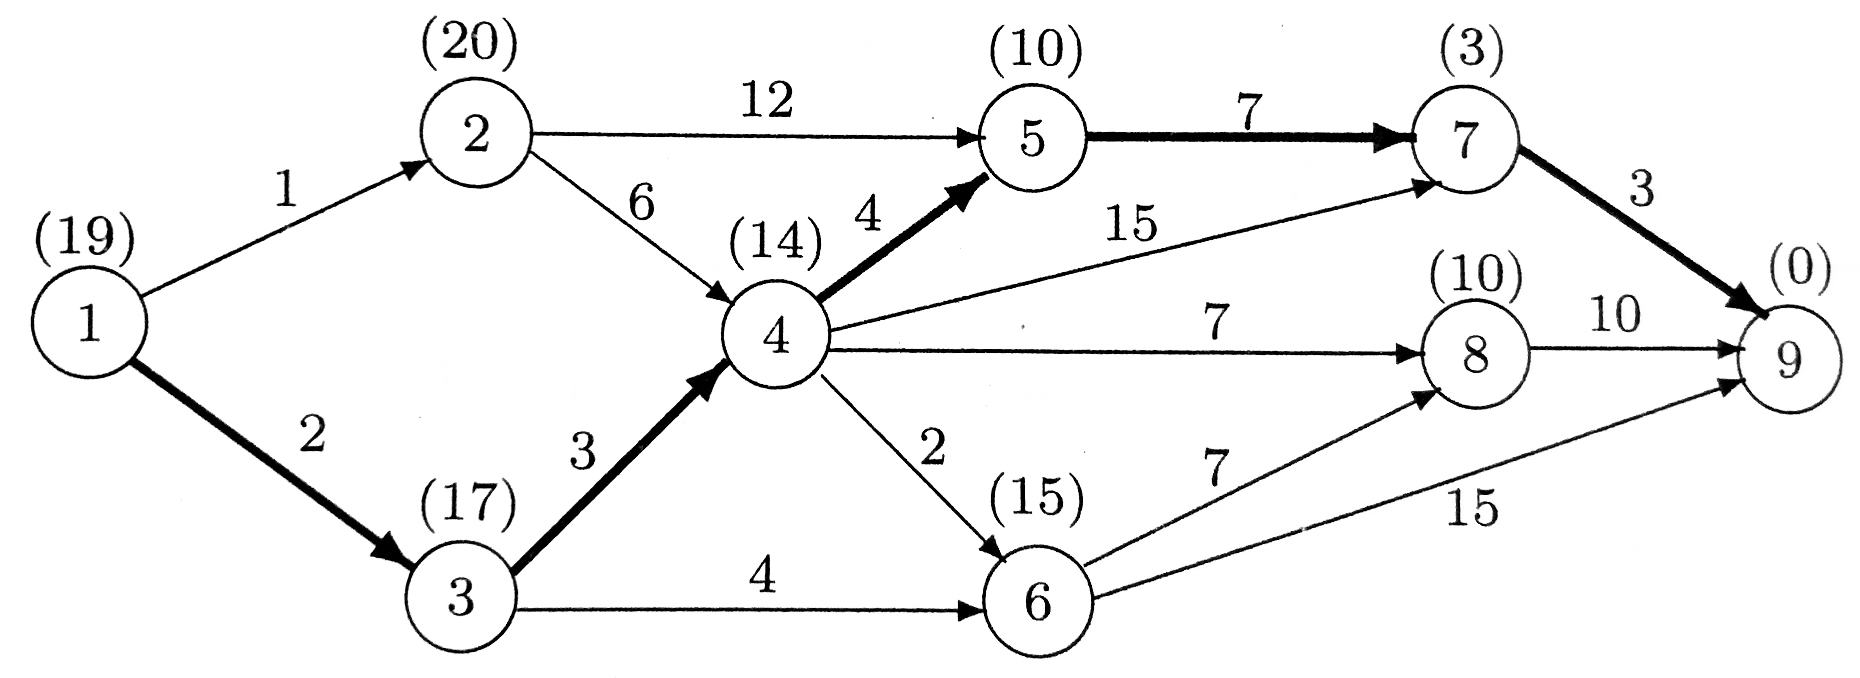
\includegraphics[width=10cm]{74.png}
  \caption{有向图最短路径问题的手工求解}
\end{figure}

\end{frame}
\begin{frame}[allowframebreaks]{有向图搜索及图示}
命令语句:

$P=biograph(R)$

$[d,p]=graphshortestpath(R,n_1,n_2)$,其中$n_1$为起点,$n_2$为终点。

例题解法:

$ab=[1 1 2 2 3 3 4 4 4 4 5 6 6 7 8];$

$bb=[2 3 5 4 4 6 5 7 8 6 7 8 9 9 9];$

$w=[1 2 12 6 3 4 4 15 7 2 7 7 15 3 10];$

R=sparse(ab,bb,w);建立关联矩阵

R(9,9)=0;

h=view(biograph(R,[],'ShowWeights','on'))显示有向图

[d,p]=graphshortestpath(R,1,9)计算最短路径,返回最短路径长度和路径节点

set(h.Nodes(p),'Color',[1 0 0])将路径节点标记成红色

\end{frame}

\begin{frame}[allowframebreaks]{有向图搜索及图示}



	\begin{columns}[T]
		\column{.45\textwidth}
    \begin{figure}[htp]
      \centering
      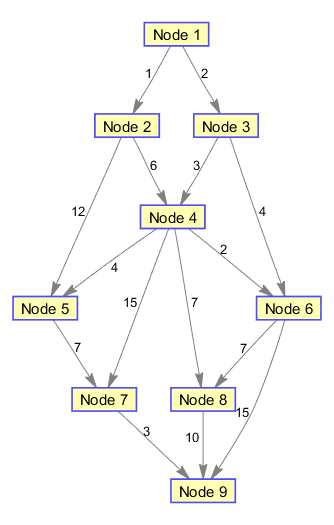
\includegraphics[width = 0.9\textwidth]{71.png}
      \caption{有向图的自动绘制}
    \end{figure}
		\column{.45\textwidth}

    \begin{figure}[htp]
      \centering
      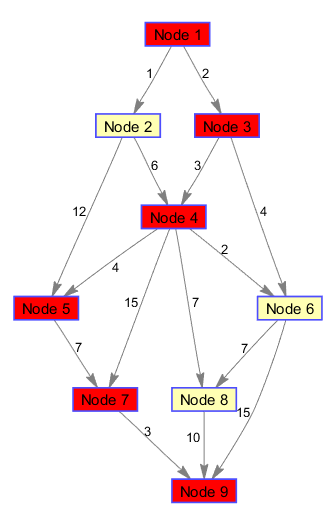
\includegraphics[width = 0.9\textwidth]{72.png}
      \caption{最短路径图形显示}
    \end{figure}
	\end{columns}

\end{frame}

\begin{frame}[allowframebreaks]{Dijkstra算法}
Dijkstra其人:

Edsger Wybe Dijkstra (04/01/1930-08/06/2002),  荷兰皇家艺术与科学学院的院士,美国科学院院士,英国计算协会的Fellow。年轻时代,Dijkstra在University of Leiden(荷兰最古老的大学)学习理论物理,但很快他就意识到其兴趣不在于理论物理虽然获得了其数学和理论物理的学位。

1984年至1999年,作为计算机系系主任任职与美国UT Austin(得克萨斯州大学奥斯汀分校),并于1999年退休。 
\begin{figure}[htp]
  \centering
  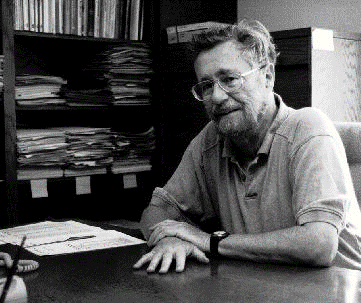
\includegraphics[width = 0.5\textwidth]{73.png}
  \caption{E. W. Dijkstra}
\end{figure}


E. W. Dijkstra 15年的学术著作覆盖了图论的理论工作,教育手册,解释文章和编程语言领域的哲学思考。

\end{frame}
\begin{frame}[allowframebreaks]{Dijkstra算法基本思路}
准备工作:

$\circ$设图G中有n个顶点,设置一个集合U存放已求出最短路径的顶点,V-U是尚未确定最短路径的顶点集合

$\circ$每个顶点对应一个距离值,则
集合U中顶点的距离值是从顶点v0到该顶点的最短路径长度;
集合V-U中顶点的距离值是从顶点v0到该顶点的只包括集合U中顶点为中间顶点的最短路径长度
\end{frame}
\begin{frame}[allowframebreaks]{Dijkstra算法基本思路}
初始状态:

$\circ$集合U中只有顶点v0,顶点v0对应的距离值为0

$\circ$集合V-U中顶点vi的距离值为边(v0,vi)的权值(i=1,…,n-1),如果v0和vi间无边直接相连,则vi的距离值为∞

在集合V-U中选择距离值最小的顶点vmin加入集合U

对集合V-U中各顶点的距离值进行修正,如果加入顶点vmin为中间顶点后,使v0到vi的距离值比原来的距离值更小,则修改vi的距离值

反复操作,直到从v0出发可以到达的所有顶点都在集合U中为止


\end{frame}
\begin{frame}[allowframebreaks]{Dijkstra算法}
function [d,path]=dijkstra(W,s,t)

[n,m]=size(W);ix=(W==0);W(ix)=Inf;

if n~=m,error('Square W required');end

visited(1:n)=0;dist(1:n)=Inf;parent(1:n)=0;dist(s)=0;d=Inf;

for i=1:(n-1),

ix=(visited==0);vec(1:n)=Inf;vec(ix)=dist(ix);

[a,u]=min(vec);visited(u)=1;

for v=1:n

if(W(u,v)+dist(u)<dist(v)),dist(v)=dist(u)+W(u,v);parent(v)=u;

end;end;end

if parent(t)~=0,path=t;d=dist(t);

while t~=s,p=parent(t);path=[p path];t=p;end

end

执行语句:[d p]=dijkstra(R,1,9)

返回:

d = 19

p = 1     3     4     5     7     9

\end{frame}

\end{document}